\documentclass{article}
\usepackage{amsmath, amsthm, amssymb, amsfonts, booktabs, hyperref, graphicx, float, esint, xcolor, subcaption, xspace, geometry}
% mathbbol, causing errors
\setlength{\abovedisplayskip}{0pt}
\setlength{\belowdisplayskip}{0pt}
\setlength{\abovedisplayshortskip}{0pt}
\setlength{\belowdisplayshortskip}{0pt}

\newcommand{\vr}{\vec{r}}
\newcommand{\vOmega}{\vec{\Omega}}
\newcommand{\vJ}{\vec{J}}
\newcommand{\vO}{\vec{\Omega}}
\newcommand{\bra}{\left\langle}
\newcommand{\ket}{\right\rangle}
\newcommand{\sbra}{\left[}
\newcommand{\sket}{\right]}
\renewcommand{\div}{\vec{\nabla} \cdot}
\newcommand{\grad}{\vec{\nabla}}
\newcommand{\vbeta}{\vec{\beta} }
\newcommand{\pdx}{\frac{\partial}{\partial x}}
\newcommand{\pdy}{\frac{\partial}{\partial y}}
\newcommand{\pdz}{\frac{\partial}{\partial z}}
\newcommand{\intrrr}{\int d^3 r \,}
\newcommand{\intrr}{\int d^2 r \,}
\newcommand{\dEdphi}{\partial_\phi E }
\newcommand{\dEdp}{\partial_p E }
\newcommand{\dBdphi}{\partial_\phi B }
\newcommand{\dBdp}{B }
\newcommand{\adj}{\phi^\dag}
\newcommand{\surf}{\int_{\partial V}}
\newcommand{\domain}{V}
\newcommand{\bound}{\partial V}
\newcommand{\vn}{\vec{n}}
\newcommand{\Edd}{\mathbb{E}}
\newcommand{\BEdd}{B}
\newcommand{\sigt}{\sigma_t}
\newcommand{\sigs}{\sigma_s}
\newcommand{\siga}{\sigma_a}
\newcommand{\isigt}{c}
% why \newcommand{\angSource}{q_\Omega}
\newcommand{\angSource}{q}
\newcommand{\scalSource}{q}
\newcommand{\angResp}{q^\dag}
\newcommand{\scalResp}{q^\dag}
\newcommand{\qoi}{{\it QoI}\xspace}


\newcommand{\comment}[2]{\marginpar{\textcolor{#2}{$\star$}}\textcolor{#2}{#1}\newline}

%-----------------------------------------------------------
%-----------------------------------------------------------
\usepackage{ifthen}
\newboolean{draftversion}
\setboolean{draftversion}{false}
%-----------------------------------------------------------
%----------------------------------------------------------

\ifthenelse{\boolean{draftversion}}
{
\newcommand{\iwh}[1]{\comment{#1}{red}}
\newcommand{\jcr}[1]{\comment{#1}{blue}}
}
{
\newcommand{\iwh}[1]{\phantom{a}}
\newcommand{\jcr}[1]{\phantom{a}}
}
\newcommand{\tcr}[1]{\comment{#1}{red}}

%%%%%%%%%%%%%%%%%%%%%%%%%%%%%%%%%%%%%%%%%%%%%%%%%%%%%%%%%%%%%%%%%%%%%%%%%%%%%%%%%%%%%%%%%%%%%%%%%%%%
%%%%%%%%%%%%%%%%%%%%%%%%%%%%%%%%%%%%%%%%%%%%%%%%%%%%%%%%%%%%%%%%%%%%%%%%%%%%%%%%%%%%%%%%%%%%%%%%%%%%
\begin{document}
\section{Blending Adjoints?}
\subsection{Sn-Transport}
So, from Sn transport, we have the following equation for the forward angular flux $\psi$,
\begin{equation}
\label{SS1GTE}
\vO \cdot \grad \psi(\vr,\vO) + \sigt(\vr) \psi(\vr,\vO) = \frac{1}{4 \pi} \sigs(\vr) \phi(\vr) + q(\vr,\vO), \quad \forall \vr \in V
\end{equation}
\begin{equation}
\label{SS1GTE_bc}
\psi(\vr,\vO) = \psi^{\text{inc}}(\vr,\vO) \quad \vr \in \partial V^{-} = \{ \vr \in \partial V, \text{ s.t. }, \vO \cdot \vec{n}(\vr) < 0\}
\end{equation}
The corresponding Sn adjoint equation,
\begin{equation}
\label{snAdj}
- \vO_d \cdot \grad \psi^\dag_d + \sigt \psi^\dag_d = \frac{\sigs}{4 \pi} \phi^\dag + \angResp_d
\end{equation}
\begin{equation}
\psi^\dag(\vr) = \psi^{\dag \text{out}}(\vr)=0 \quad \vr \in \partial V^{+} = \{  \vr \in \bound , \quad \vO \cdot \vec{n} > 0 \}
\end{equation}
and the sensitivity inner product
\begin{equation}
\label{snSens}
\begin{split}
\delta QoI &= \bra \delta \scalSource - \delta \sigt \psi + \frac{\delta\sigs}{4 \pi} \phi  , \psi^\dag  \ket - \sbra \delta \psi, \psi^\dag \sket \\
&= \bra \delta \scalSource - \delta \sigt \psi + \frac{\delta\sigs}{4 \pi} \phi , \psi^\dag  \ket - \sbra \delta \psi^{\text{inc}}, \psi^\dag \sket_- \,.
\end{split}
\end{equation}

\subsection{VET Method}
Application of the VET method gives an equation for the scalar flux. It is important to remember that this is the true, physical scalar flux of the system.
\begin{equation}
\label{VEFForm}
- \div \left( \frac{1}{\sigt}\div \Edd \phi \right) + \siga \phi = \scalSource \,
\end{equation}
\begin{equation}
2 J^{\text{inc}}(\vr) = \BEdd(\vr) \phi(\vr) + \vn \cdot \frac{1}{\sigt} \div \Edd \phi \,.
\end{equation}
And a corresponding adjoint. I have chosen to use $\varphi^\dag$ for the adjoint, as it bares no direct relation to adjoint term in the Sn scheme $\phi^\dag$
\begin{equation}
\label{adjForm}
- \Edd : \left( \grad \left( \frac{1}{\sigt}\grad \varphi^\dag \right) \right) + \siga \varphi^\dag = \scalResp
\end{equation}
\begin{equation}
\label{adjVETBC}
2J^{\dag,\text{out}} = B \varphi^\dag + 
\Edd \cdot \frac{1}{\sigma_{t} } \vec{\nabla} \varphi^\dag   \quad \vr \in \bound
\end{equation}
Leading to the sensitivity (ignoring $\delta \Edd$ perturbations).
\begin{equation}
\delta \qoi = \bra \delta q , \varphi^\dag \ket - \bra \delta c \grad \Edd \phi, \div \varphi^\dag \ket + \bra \delta \sigma_a \phi, \varphi^\dag \ket - \sbra \delta \phi, 2J^{\dag,\text{out}} \sket + \sbra \phi^\dag, 2 \delta J_p^{\text{inc}} \sket
\end{equation}

\subsection{Combining methods}
So, now there are two direct ways to proceed with sensitivity calculations. First is to do a forward SN solve, and adjoint SN solve, store both $\psi$ and $\psi^\dag$ and use the first sensitivity expression. This is the more accurate method, but involves storing off the massive angular flux data.

The other direct method is to perform a forward SN solve, save off $\phi$ and $\Edd$, then perform a VET solve for $\varphi^\dag$ and perform the sensitivity calculations using the VET method. But we lose accurate due to the $\delta \Edd$ terms.

However if our forward source and cross sections are isotropic, it may be possible to blend the two above into a form.
\begin{equation}
\delta \qoi = \bra \delta q , \phi^\dag \ket - \bra \delta c \grad \Edd \phi, \div \varphi^\dag \ket + \bra \delta \sigma_a \phi, \varphi^\dag \ket - \sbra \delta \psi^{\text{inc}}, \psi^\dag \sket_-
\end{equation}
This requires two forward Sn solves for $\psi$ and $\psi^\dag$, but only save off $\phi$, $\phi^\dag$, and $\Edd$ as well as optionally $\psi^{\dag,inc}$ on the boundary. Then do a VET solve to get $\varphi^\dag$. The above is using the Sn adjoint flux for source sensitivities (which should be exact), but the VET adjoint for cross-section sensitivities (which means we do not need to store $\psi$ and $\psi^\dag$).

\section{Eddington term}
Terms of the form below show up frequently
\begin{equation}
\div \isigt \div \left( \Edd \phi \right)
\end{equation}
Manipulate this a bit using product rule
\begin{equation}
\begin{split}
& \div \isigt \div \left( \Edd \phi \right) \\
& \div \isigt  \left( \phi (\div \Edd) + (\grad \phi) \cdot \Edd \right) \\
& \div \isigt  \left( \phi (\div \Edd) \left) + \div \isigt\right( (\grad \phi) \cdot \Edd \right) \\
& \div \isigt  \left( (\div \Edd) \phi  \left) + \div \isigt\right( \Edd^T (\grad \phi) \right) \\
&  \isigt  \left( (\div \div \Edd) \phi + \grad \phi \cdot  (\div \Edd) \left) + \div \isigt\right( \Edd^T (\grad \phi) \right) \\
\end{split}
\end{equation}

(drop the factor of $\isigt$ for a sec) Above is somewhat in the form of a diffusion/convection system
\begin{equation}
\begin{split}
&    \div \left( \Edd^T (\grad \phi) \right) + (\div \Edd)^T \grad \phi  +   (\div \div \Edd) \phi\\
\end{split}
\end{equation}

\section{Some results}
\newgeometry{left=0.5cm,,right=0.1cm,bottom=0.5cm}
\newpage
\subsection{19}
\begin{verbatim}
    case 19 %Uniform, 0 inc flux. Response in middle
        % number of elements per zone
        nel_zone = [ 10 10 10 10 10]*4;
        % width of each zone
        width_zone = [ 2 2 2 2 2];
        % sigt/sigs per zone
        sigt=[2 2 2 2 2];
        sigs=[1 1 1 1 1];
        % volumetric source value, per zone
        qvf=[1 1 1 1 1];
        % incoming flux values
        incf(1:sn) = 0;
        % volumetric response value, per zone
        qva=[0 0 1 0 0];
        % incoming adj flux values
        inca(1:sn) = 0;
        %Regions to be perturbed. Use value of 1 to specify
        dat.sigaPertRegion=[1 1 1 1 1];
        dat.sigsPertRegion=[1 1 1 1 1];
        dat.sourcePertRegion=[1 1 1 1 1];
        dat.incPertRegion(1:sn)=1;
        
-----BEGIN UNPERTURBED QOI DATA OUTPUT----- 
qoi using sn forward: 	 1.99988 
qoi using sn adjoint: 	 1.99988 
qoi using VEFforward: 	 1.99988 
qoi using VEF math adj: 	 1.99988 
\end{verbatim}

\begin{figure}[H]
\label{InHomoPertq}
\centering
\begin{subfigure}{.5\textwidth}
  \centering
  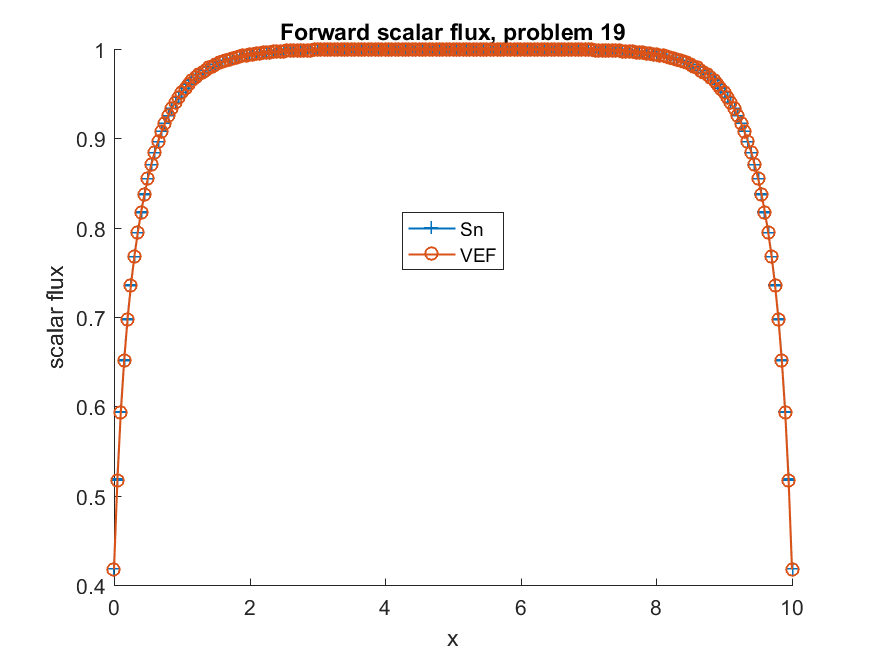
\includegraphics[width=.98\linewidth]{IanProposal/figures2/19phi.png}
  \caption{Forward flux}
  \label{fig:sfig1}
\end{subfigure}%
\begin{subfigure}{.5\textwidth}
  \centering
  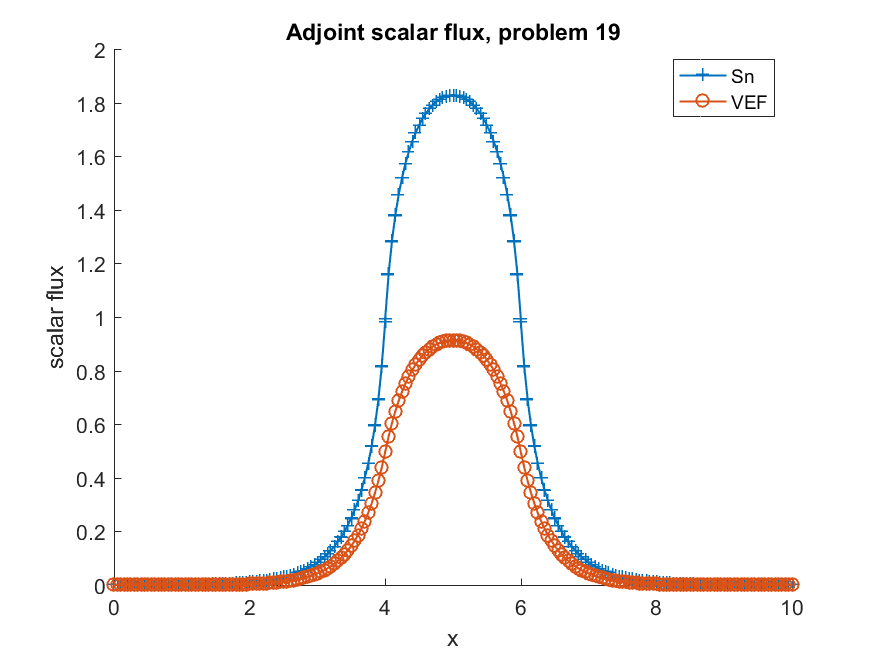
\includegraphics[width=.98\linewidth]{IanProposal/figures2/19phia.png}
  \caption{Response flux}
  \label{fig:sfig4}
\end{subfigure}%
\end{figure}


\begin{figure}[H]
\label{InHomoPertq}
\centering
\begin{subfigure}{.5\textwidth}
  \centering
  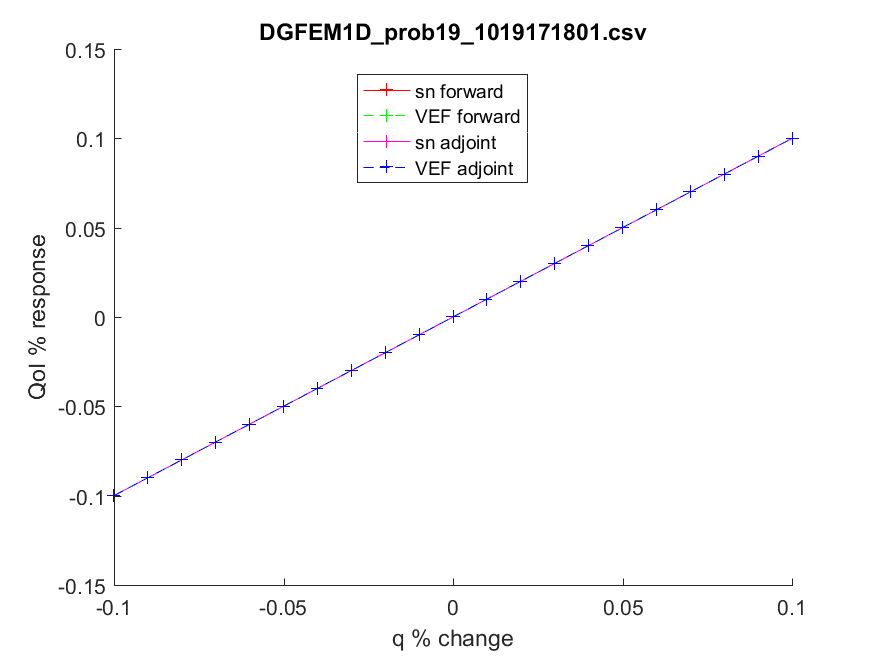
\includegraphics[width=.98\linewidth]{IanProposal/figures2/19qSens.png}
  \caption{Source sensitivity}
  \label{fig:sfig1}
\end{subfigure}%
\begin{subfigure}{.5\textwidth}
  \centering
  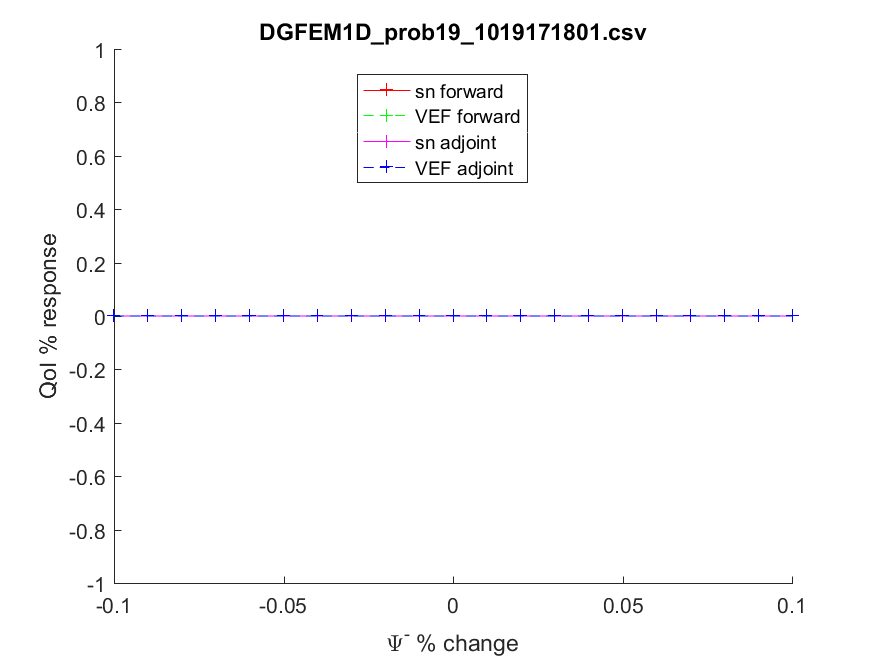
\includegraphics[width=.98\linewidth]{IanProposal/figures2/19incSens.png}
  \caption{Incident flux sensitivity}
  \label{fig:sfig4}
\end{subfigure}%
\\
\begin{subfigure}{.5\textwidth}
  \centering
  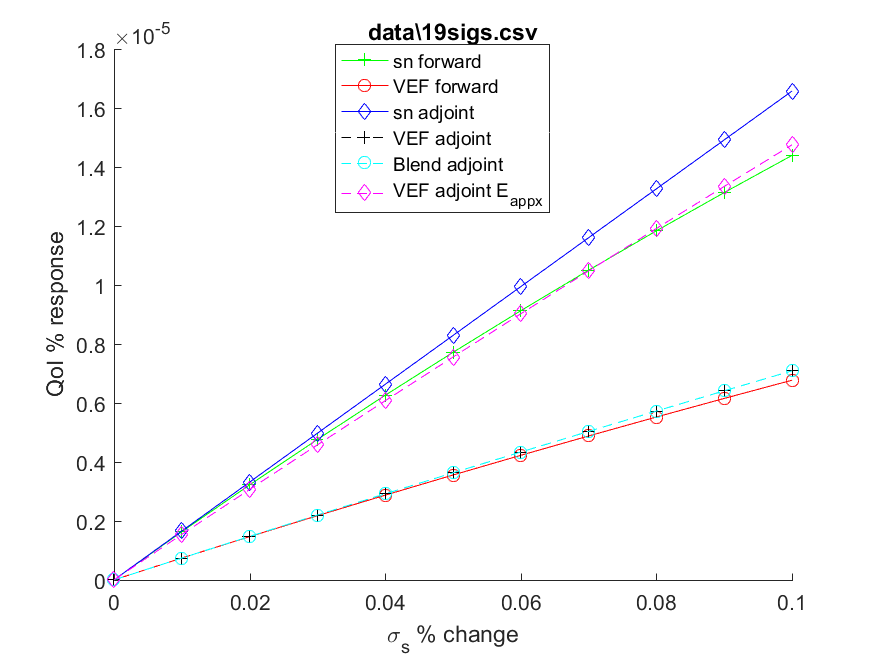
\includegraphics[width=.98\linewidth]{IanProposal/figures2/19sigsSens.png}
  \caption{Scattering cross-section sensitivity}
  \label{fig:sfig2}
\end{subfigure}%
\begin{subfigure}{.5\textwidth}
  \centering
  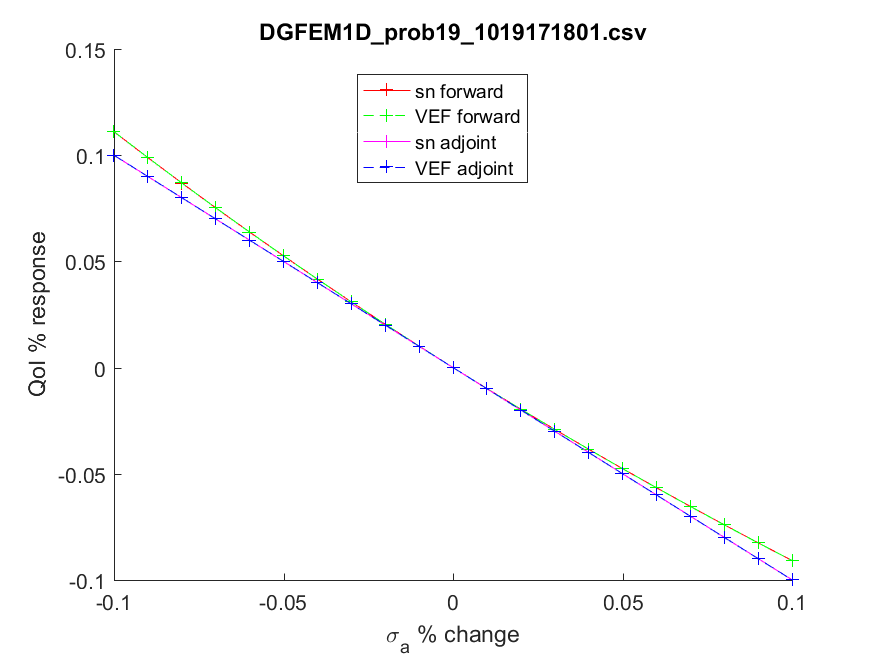
\includegraphics[width=.98\linewidth]{IanProposal/figures2/19sigaSens.png}
  \caption{Absorption cross-section sensitivity}
  \label{fig:sfig5}
\end{subfigure}%
\caption{}
\label{fig:fig}
\end{figure}
\newpage

%%%%%%%%%%%%%%%%%%%%%%%%%%%%%%%%%%%%%%%%%%%%%%%%%%%%%%
%%%%%%%%%%%%%%%%%%%%%%%%%%%%%%%%%%%%%%%%%%%%%%%%%%%%%%
%%%%%%%%%%%%%%%%%%%%%%%%%%%%%%%%%%%%%%%%%%%%%%%%%%%%%%
\subsection{60. Scat to vac}
\begin{verbatim}
case 60 %
        % number of elements per zone
        nel_zone = [ 10 10 10 10 10 10]*4;
        % width of each zone
        width_zone = [1 1 1 1 1 1];
        % sigt/sigs per zone
        sigt=[1 1 1 1e-8 1e-8 1e-8];
        sigs=[1 1 1 0 0 0];
        % volumetric source value, per zone
        qvf=[0 0 0 0 0 0];
        % incoming flux values
        incf(1:sn) = 0;
        incf((sn/2)+1:sn) = 1;
        % volumetric response value, per zone
        qva=[0 0 1 1 0 0];
        % incoming adj flux values
        inca(1:sn) = 0;
        %Regions to be perturbed. Use value of 1 to specify
        dat.sigaPertRegion=[0 0 0 0 0 0];
        dat.sigsPertRegion=[1 1 1 0 0 0];
        dat.sourcePertRegion=[0 0 0 0 0 0];
        dat.incPertRegion(1:sn) = 1;
        
-----BEGIN UNPERTURBED QOI DATA OUTPUT----- 
qoi using sn forward: 	 0.789965 
qoi using sn adjoint: 	 0.789965 
qoi using VEF forward: 	 0.78984 
qoi using VEF adjoint: 	 0.78984 
\end{verbatim}

\begin{figure}[H]
\label{Case60Flux}
\centering
\begin{subfigure}{.5\textwidth}
  \centering
  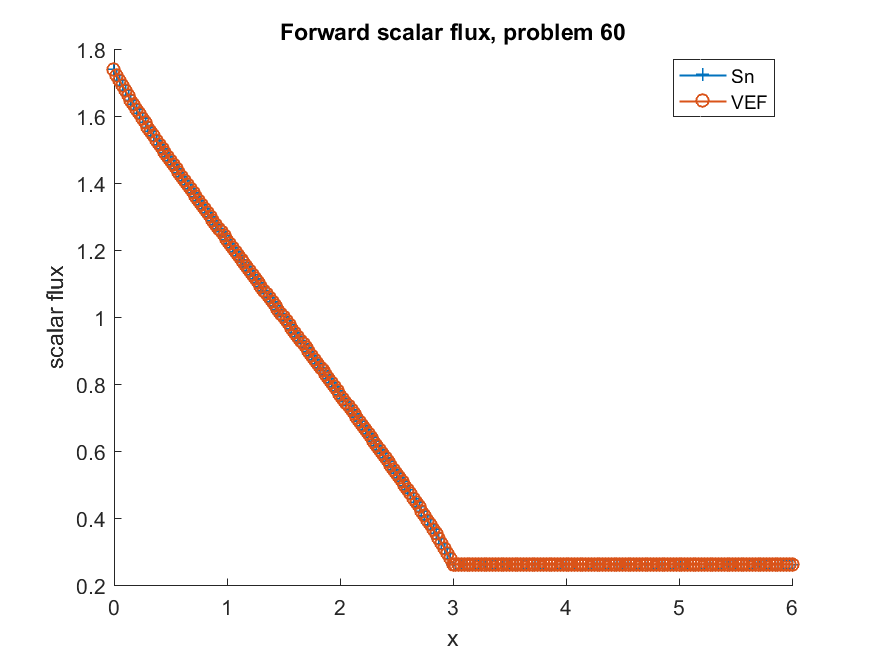
\includegraphics[width=.98\linewidth]{IanProposal/figures2/60phi.png}
  \caption{Forward flux}
  \label{fig:sfig1}
\end{subfigure}%
\begin{subfigure}{.5\textwidth}
  \centering
  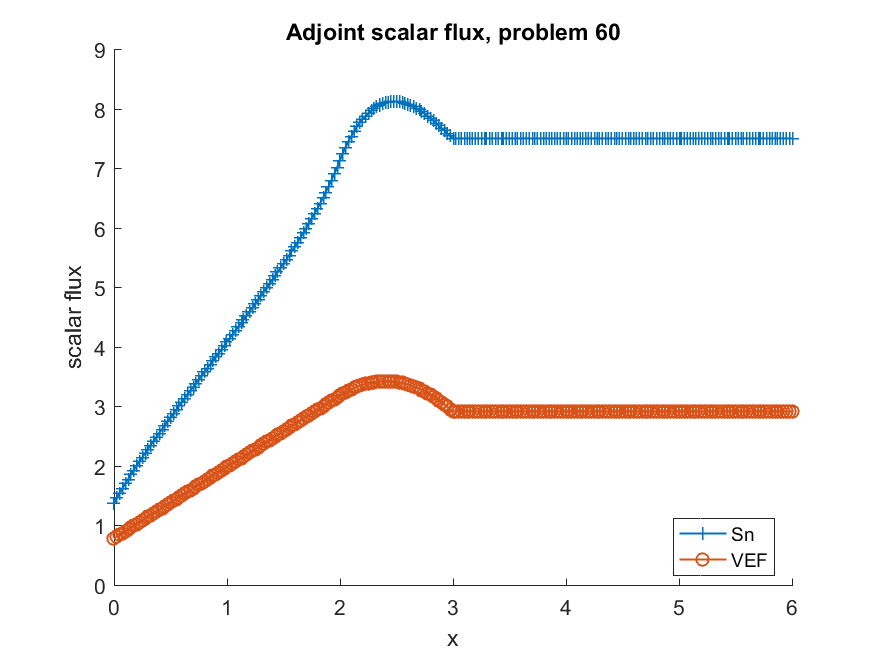
\includegraphics[width=.98\linewidth]{IanProposal/figures2/60phia.png}
  \caption{Response flux}
  \label{fig:sfig4}
\end{subfigure}%
\end{figure}


\begin{figure}[H]
\label{Case60Sens}
\centering
\begin{subfigure}{.5\textwidth}
  \centering
  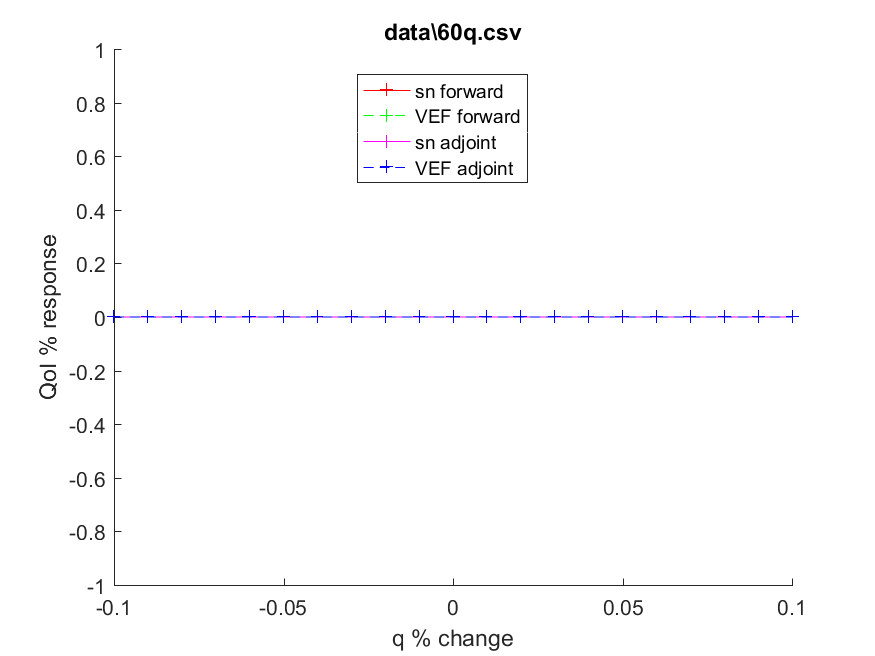
\includegraphics[width=.98\linewidth]{IanProposal/figures2/60qSens.png}
  \caption{Source sensitivity}
  \label{fig:sfig1}
\end{subfigure}%
\begin{subfigure}{.5\textwidth}
  \centering
  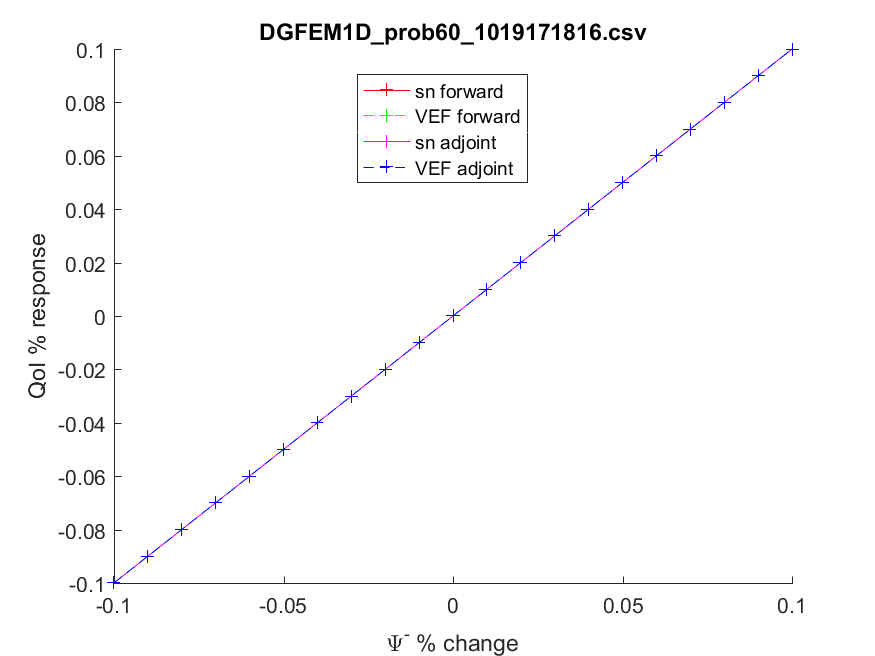
\includegraphics[width=.98\linewidth]{IanProposal/figures2/60incSens.png}
  \caption{Incident flux sensitivity}
  \label{fig:sfig4}
\end{subfigure}%
\\
\begin{subfigure}{.5\textwidth}
  \centering
  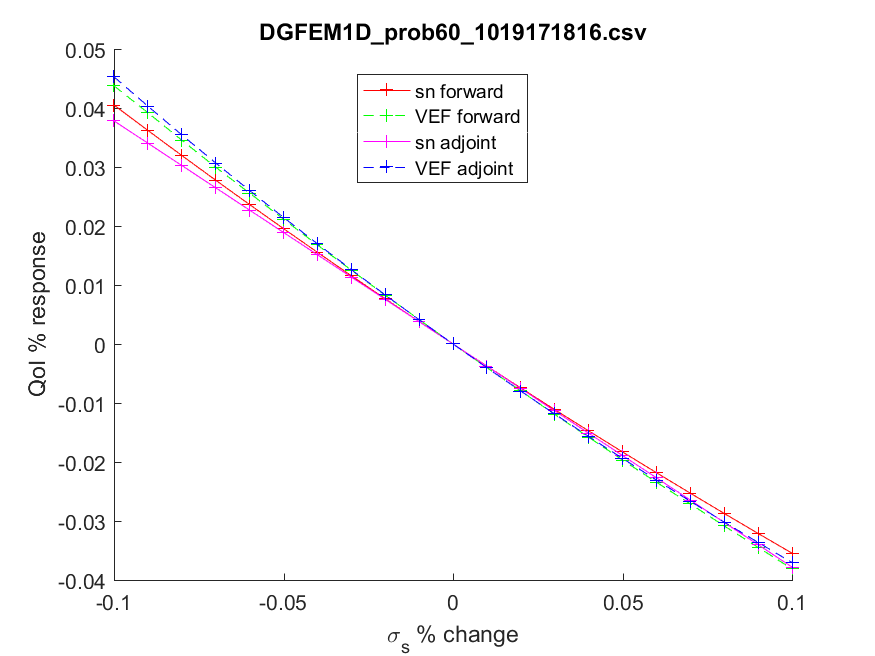
\includegraphics[width=.98\linewidth]{IanProposal/figures2/60sigsSens.png}
  \caption{Scattering cross-section sensitivity}
  \label{fig:sfig2}
\end{subfigure}%
\begin{subfigure}{.5\textwidth}
  \centering
  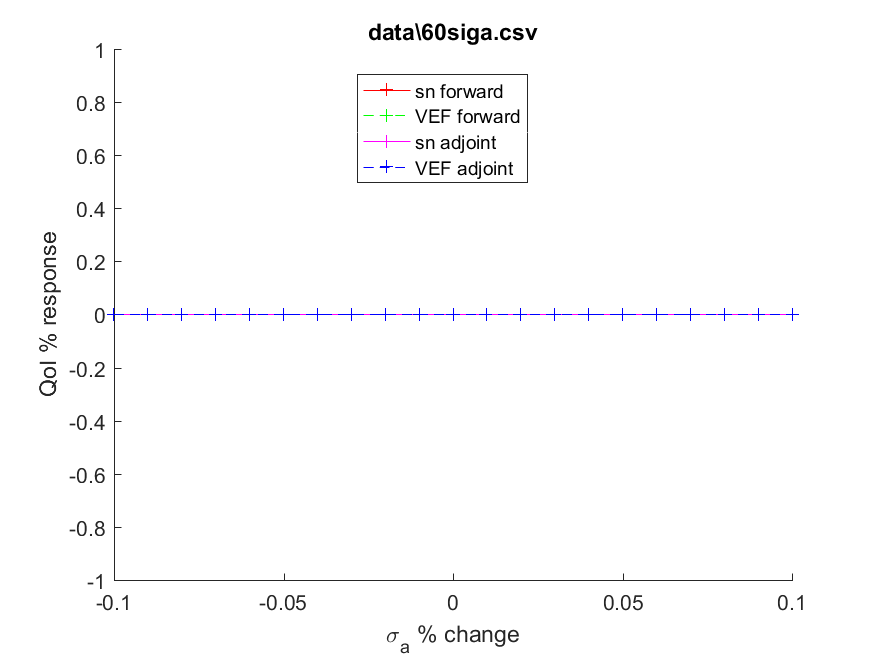
\includegraphics[width=.98\linewidth]{IanProposal/figures2/60sigaSens.png}
  \caption{Absorption cross-section sensitivity}
  \label{fig:sfig5}
\end{subfigure}%
\caption{}
\label{fig:fig}
\end{figure}
\newpage

%%%%%%%%%%%%%%%%%%%%%%%%%%%%%%%%%%%%%%%%%%%%%%%%%%%%%%
%%%%%%%%%%%%%%%%%%%%%%%%%%%%%%%%%%%%%%%%%%%%%%%%%%%%%%
%%%%%%%%%%%%%%%%%%%%%%%%%%%%%%%%%%%%%%%%%%%%%%%%%%%%%%
\subsection{61. Scat to vac}
\begin{verbatim}
case 61 %
        % number of elements per zone
        nel_zone = [ 10 10 10 10 10 10]*4;
        % width of each zone
        width_zone = [1 1 1 1 1 1];
        % sigt/sigs per zone
        sigt=[1 1 1 1e-8 1e-8 1e-8];
        sigs=[1 1 1 0 0 0];
        % volumetric source value, per zone
        qvf=[0 0 0 0 0 0];
        % incoming flux values
        incf(1:sn) = 0;
        incf((sn/2)+1:sn) = 1;
        % volumetric response value, per zone
        qva=[0 1 1 0 0 0];
        % incoming adj flux values
        inca(1:sn) = 0;
        %Regions to be perturbed. Use value of 1 to specify
        dat.sigaPertRegion=[0 0 0 0 0 0];
        dat.sigsPertRegion=[1 1 1 0 0 0];
        dat.sourcePertRegion=[0 0 0 0 0 0];
        dat.incPertRegion(1:sn) = 1;
        
-----BEGIN UNPERTURBED QOI DATA OUTPUT----- 
qoi using sn forward: 	 1.5282 
qoi using sn adjoint: 	 1.5282 
qoi using VEF forward: 	 1.5281 
qoi using VEF adjoint: 	 1.5281 
\end{verbatim}

\begin{figure}[H]
\label{Case61Flux}
\centering
\begin{subfigure}{.5\textwidth}
  \centering
  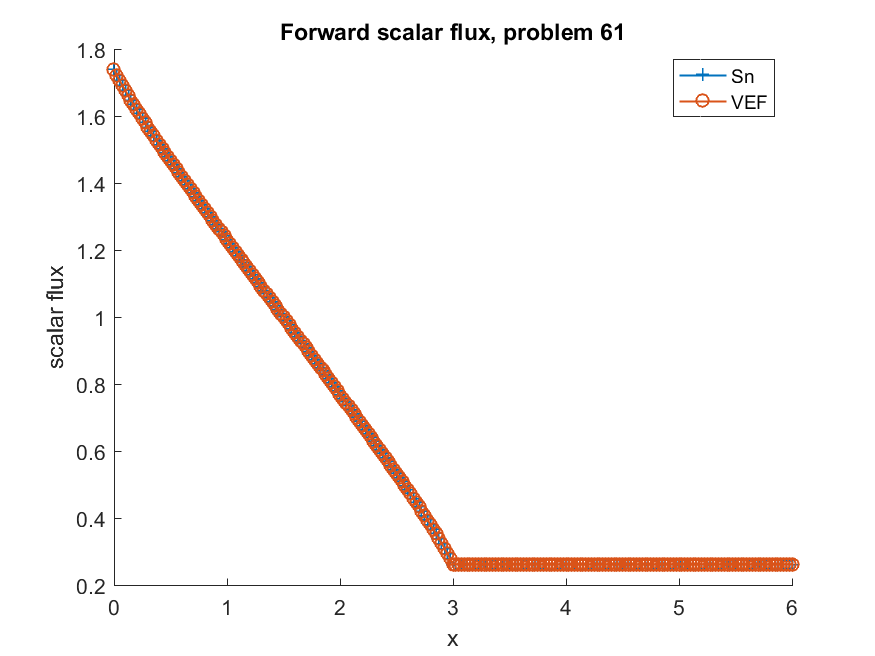
\includegraphics[width=.98\linewidth]{IanProposal/figures2/61phi.png}
  \caption{Forward flux}
  \label{fig:sfig1}
\end{subfigure}%
\begin{subfigure}{.5\textwidth}
  \centering
  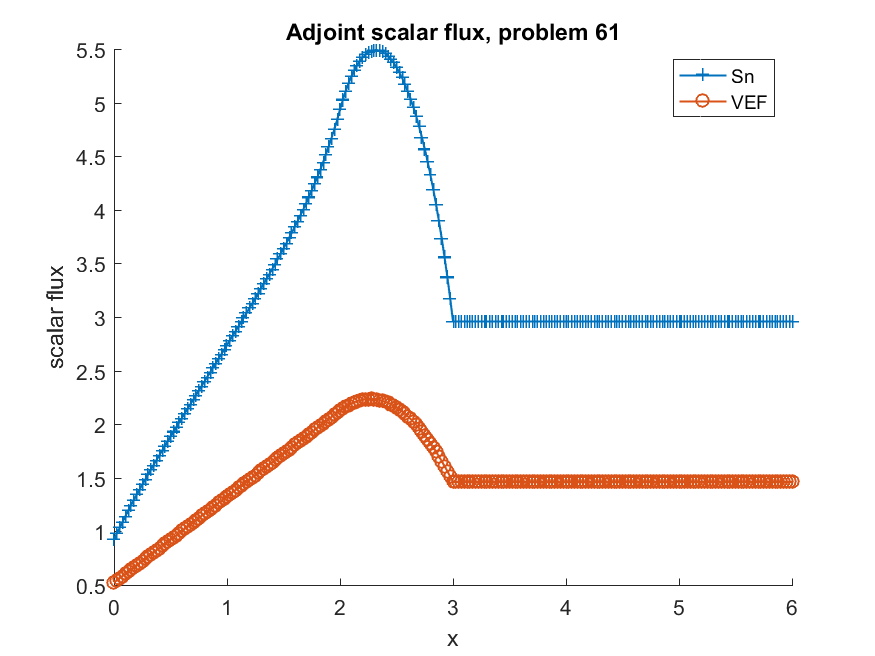
\includegraphics[width=.98\linewidth]{IanProposal/figures2/61phia.png}
  \caption{Response flux}
  \label{fig:sfig4}
\end{subfigure}%
\end{figure}


\begin{figure}[H]
\label{Case61Sens}
\centering
\begin{subfigure}{.5\textwidth}
  \centering
  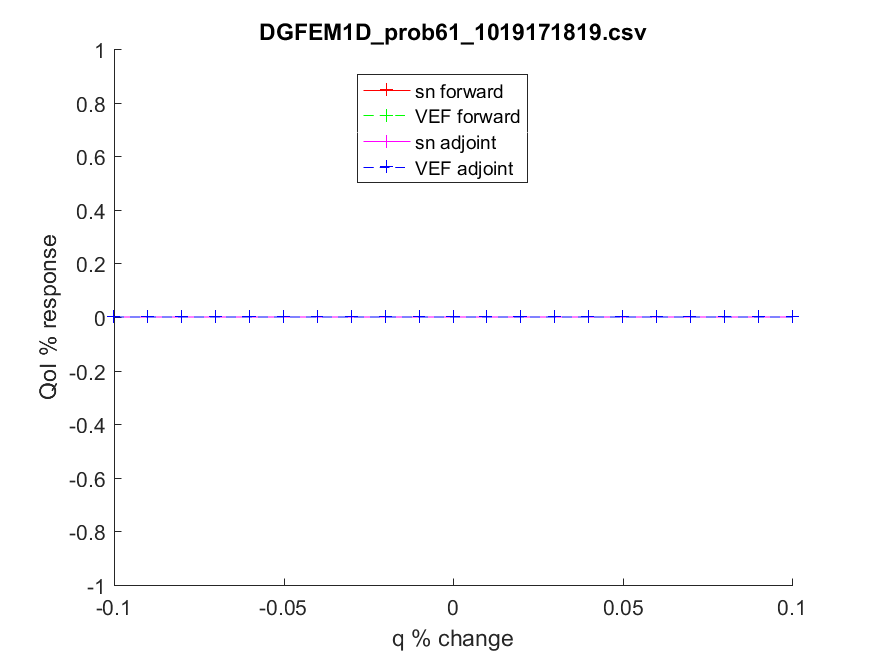
\includegraphics[width=.98\linewidth]{IanProposal/figures2/61qSens.png}
  \caption{Source sensitivity}
  \label{fig:sfig1}
\end{subfigure}%
\begin{subfigure}{.5\textwidth}
  \centering
  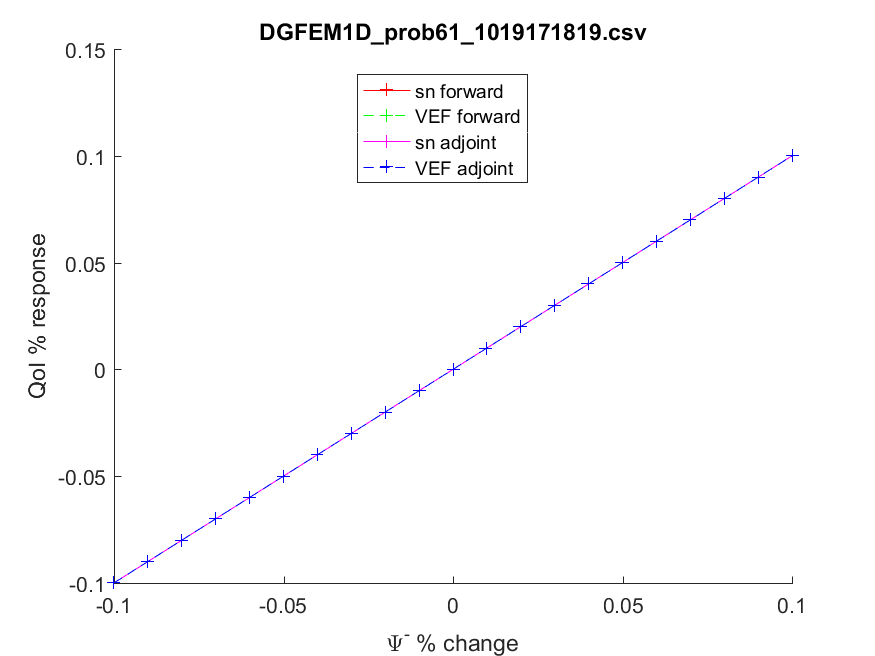
\includegraphics[width=.98\linewidth]{IanProposal/figures2/61incSens.png}
  \caption{Incident flux sensitivity}
  \label{fig:sfig4}
\end{subfigure}%
\\
\begin{subfigure}{.5\textwidth}
  \centering
  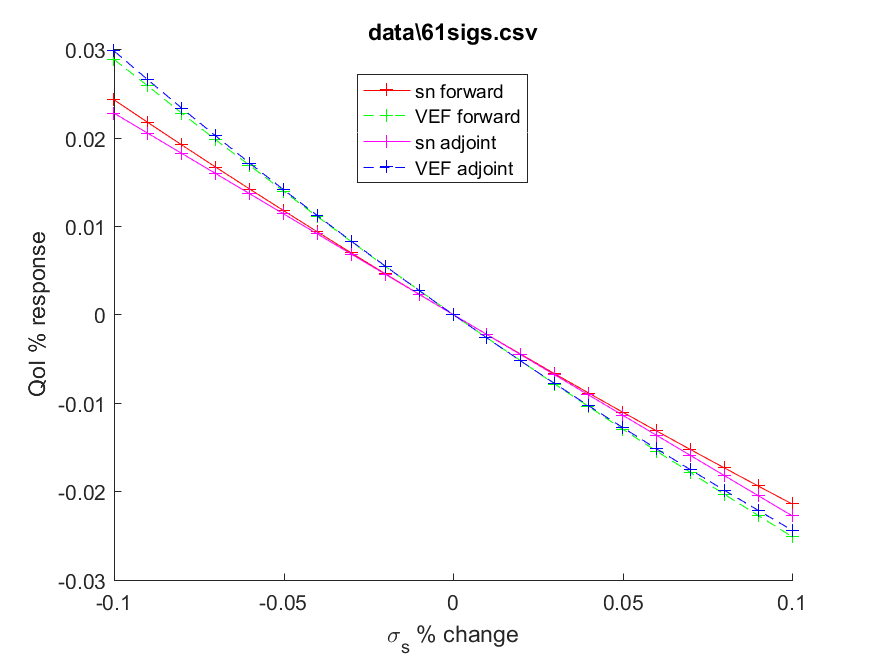
\includegraphics[width=.98\linewidth]{IanProposal/figures2/61sigsSens.png}
  \caption{Scattering cross-section sensitivity}
  \label{fig:sfig2}
\end{subfigure}%
\begin{subfigure}{.5\textwidth}
  \centering
  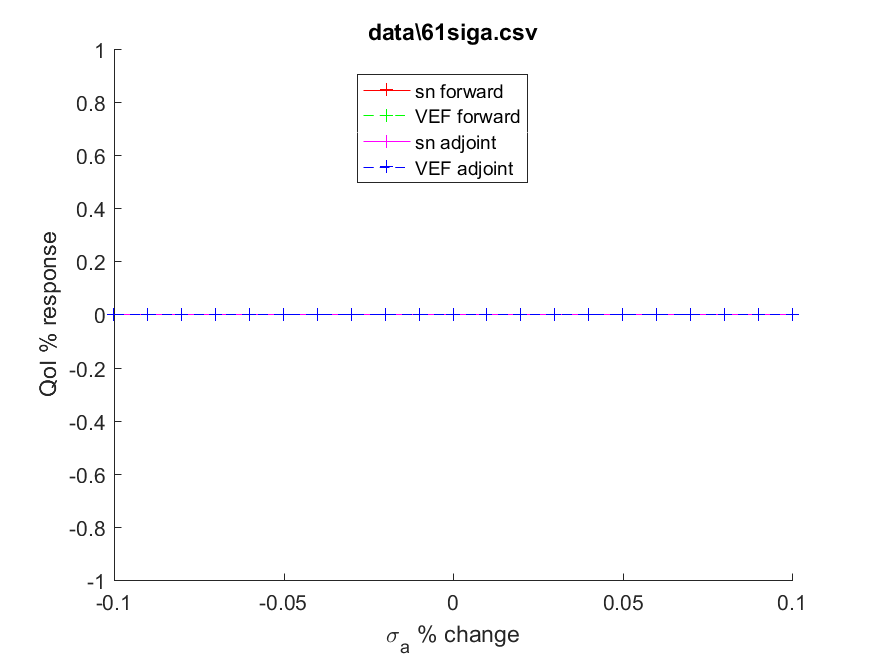
\includegraphics[width=.98\linewidth]{IanProposal/figures2/61sigaSens.png}
  \caption{Absorption cross-section sensitivity}
  \label{fig:sfig5}
\end{subfigure}%
\caption{}
\label{fig:fig}
\end{figure}
\newpage

%%%%%%%%%%%%%%%%%%%%%%%%%%%%%%%%%%%%%%%%%%%%%%%%%%%%%%
%%%%%%%%%%%%%%%%%%%%%%%%%%%%%%%%%%%%%%%%%%%%%%%%%%%%%%
%%%%%%%%%%%%%%%%%%%%%%%%%%%%%%%%%%%%%%%%%%%%%%%%%%%%%%
\subsection{62. Scat to vac}
\begin{verbatim}
case 62 %
        % number of elements per zone
        nel_zone = [ 10 10 10 10 10 10]*4;
        % width of each zone
        width_zone = [1 1 1 1 1 1];
        % sigt/sigs per zone
        sigt=[1 1 1 1e-8 1e-8 1e-8];
        sigs=[1 1 1 0 0 0];
        % volumetric source value, per zone
        qvf=[0 0 0 0 0 0];
        % incoming flux values
        incf(1:sn) = 0;
        incf((sn/2)+1:sn) = 1;
        % volumetric response value, per zone
        qva=[0 0 0 1 1 0];
        % incoming adj flux values
        inca(1:sn) = 0;
        %Regions to be perturbed. Use value of 1 to specify
        dat.sigaPertRegion=[0 0 0 0 0 0];
        dat.sigsPertRegion=[1 1 1 0 0 0];
        dat.sourcePertRegion=[0 0 0 0 0 0];
        dat.incPertRegion(1:sn) = 1;
        
-----BEGIN UNPERTURBED QOI DATA OUTPUT----- 
qoi using sn forward: 	 0.52354 
qoi using sn adjoint: 	 0.52354 
qoi using VEF forward: 	 0.523413 
qoi using VEF adjoint: 	 0.523413 
\end{verbatim}

\begin{figure}[H]
\label{Case62Flux}
\centering
\begin{subfigure}{.5\textwidth}
  \centering
  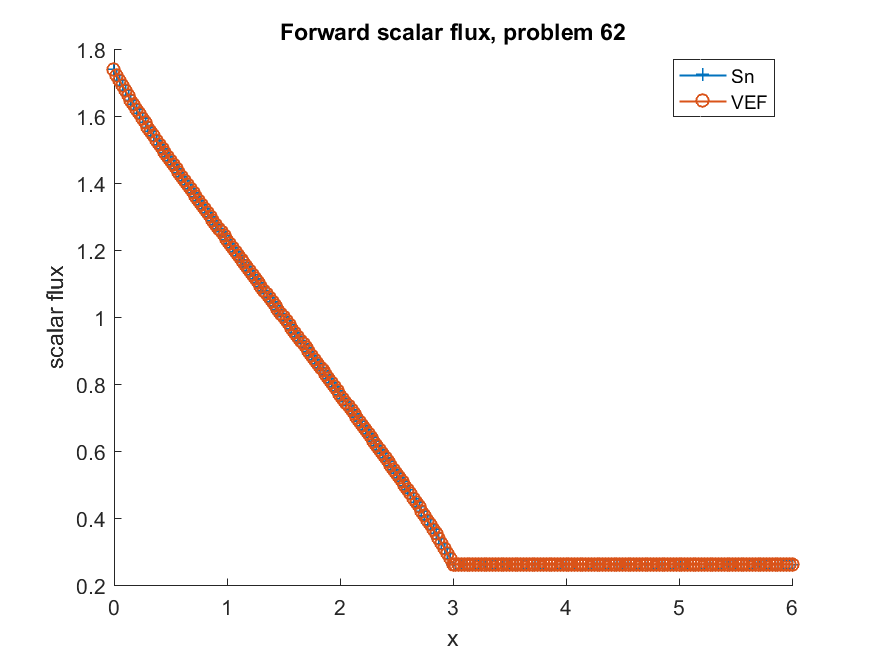
\includegraphics[width=.98\linewidth]{IanProposal/figures2/62phi.png}
  \caption{Forward flux}
  \label{fig:sfig1}
\end{subfigure}%
\begin{subfigure}{.5\textwidth}
  \centering
  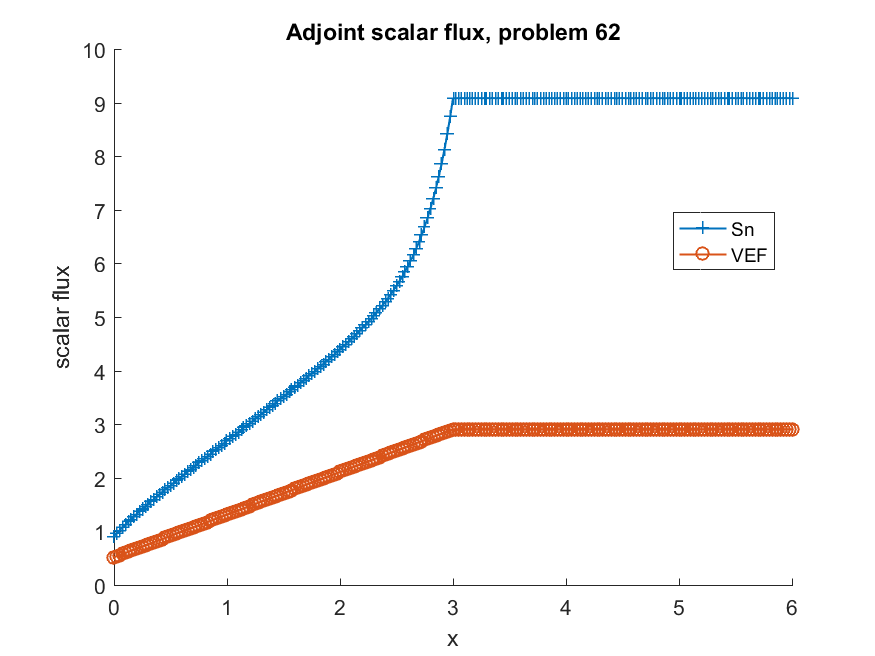
\includegraphics[width=.98\linewidth]{IanProposal/figures2/62phia.png}
  \caption{Response flux}
  \label{fig:sfig4}
\end{subfigure}%
\end{figure}


\begin{figure}[H]
\label{Case62Sens}
\centering
\begin{subfigure}{.5\textwidth}
  \centering
  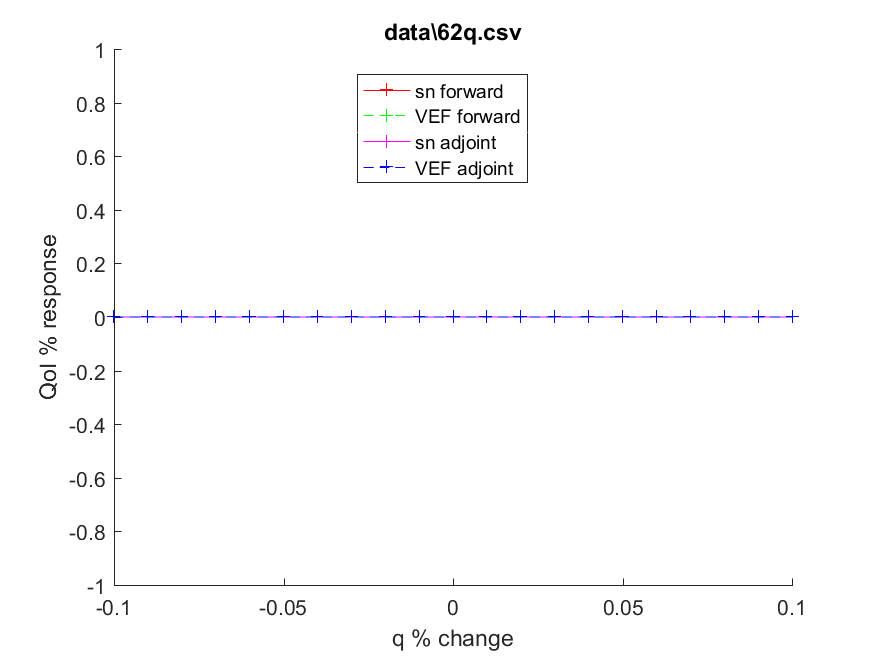
\includegraphics[width=.98\linewidth]{IanProposal/figures2/62qSens.png}
  \caption{Source sensitivity}
  \label{fig:sfig1}
\end{subfigure}%
\begin{subfigure}{.5\textwidth}
  \centering
  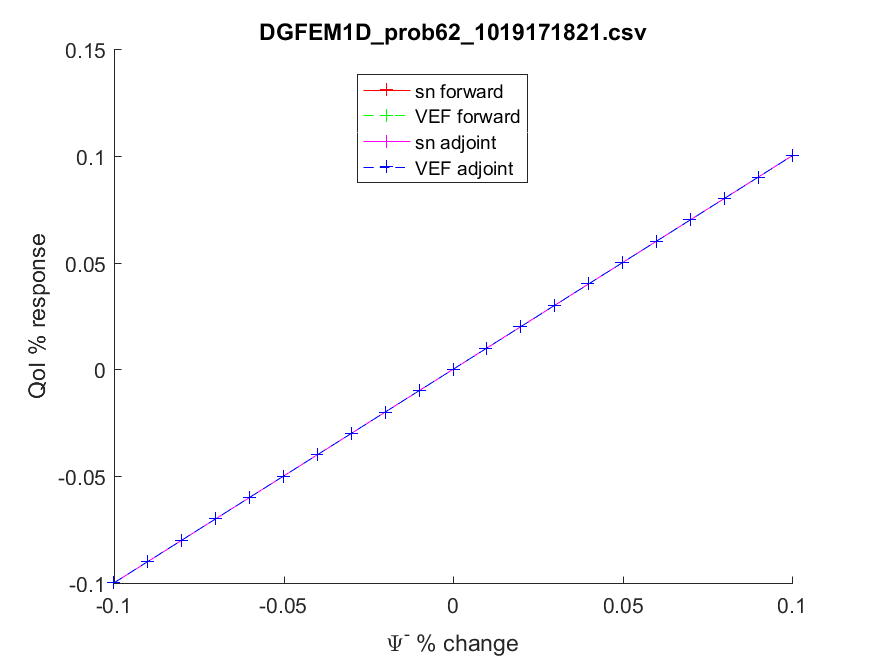
\includegraphics[width=.98\linewidth]{IanProposal/figures2/62incSens.png}
  \caption{Incident flux sensitivity}
  \label{fig:sfig4}
\end{subfigure}%
\\
\begin{subfigure}{.5\textwidth}
  \centering
  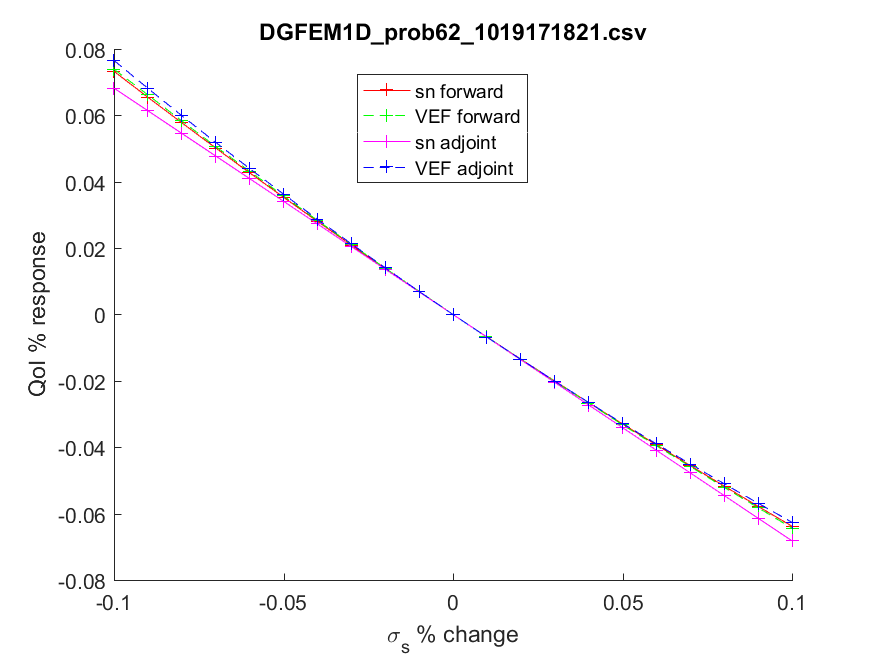
\includegraphics[width=.98\linewidth]{IanProposal/figures2/62sigsSens.png}
  \caption{Scattering cross-section sensitivity}
  \label{fig:sfig2}
\end{subfigure}%
\begin{subfigure}{.5\textwidth}
  \centering
  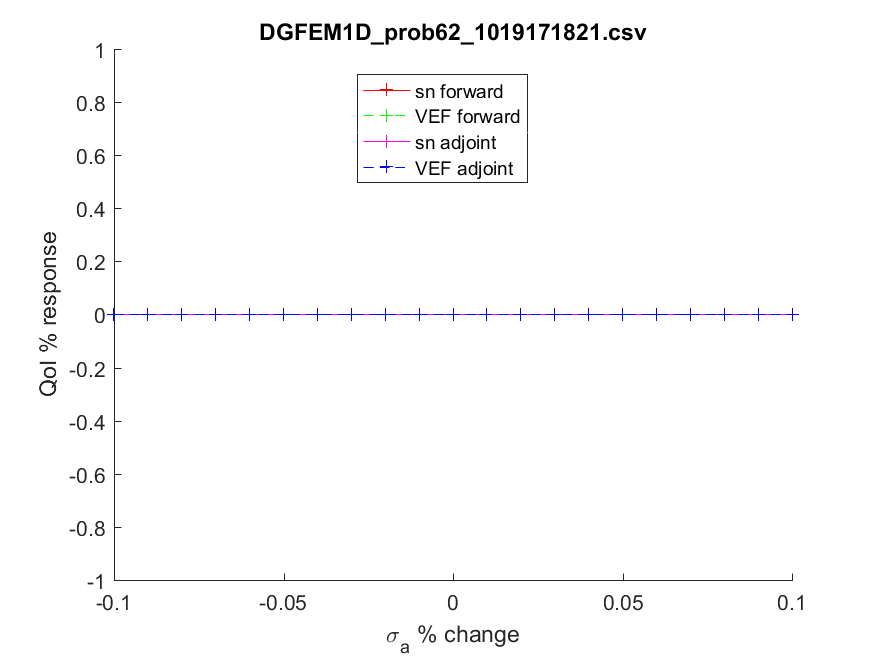
\includegraphics[width=.98\linewidth]{IanProposal/figures2/62sigaSens.png}
  \caption{Absorption cross-section sensitivity}
  \label{fig:sfig5}
\end{subfigure}%
\caption{}
\label{fig:fig}
\end{figure}
\newpage

%%%%%%%%%%%%%%%%%%%%%%%%%%%%%%%%%%%%%%%%%%%%%%%%%%%%%%
%%%%%%%%%%%%%%%%%%%%%%%%%%%%%%%%%%%%%%%%%%%%%%%%%%%%%%
%%%%%%%%%%%%%%%%%%%%%%%%%%%%%%%%%%%%%%%%%%%%%%%%%%%%%%
\subsection{63. Scat to abs}
\begin{verbatim}
case 63 %
        % number of elements per zone
        nel_zone = [ 10 10 10 10 10 10]*4;
        % width of each zone
        width_zone = [1 1 1 1 1 1];
        % sigt/sigs per zone
        sigt=[1 1 1 1 1 1];
        sigs=[1 1 1 0 0 0];
        % volumetric source value, per zone
        qvf=[0 0 0 0 0 0];
        % incoming flux values
        incf(1:sn) = 0;
        incf((sn/2)+1:sn) = 1;
        % volumetric response value, per zone
        qva=[0 0 1 1 0 0];
        % incoming adj flux values
        inca(1:sn) = 0;
        %Regions to be perturbed. Use value of 1 to specify
        dat.sigaPertRegion=[0 0 0 1 1 1];
        dat.sigsPertRegion=[1 1 1 0 0 0];
        dat.sourcePertRegion=[0 0 0 0 0 0];
        dat.incPertRegion(1:sn) = 1; 
        
-----BEGIN UNPERTURBED QOI DATA OUTPUT----- 
qoi using sn forward: 	 0.643203 
qoi using sn adjoint: 	 0.643203 
qoi using VEF forward: 	 0.643198 
qoi using VEF adjoint: 	 0.643198 
\end{verbatim}

\begin{figure}[H]
\label{Case63Flux}
\centering
\begin{subfigure}{.5\textwidth}
  \centering
  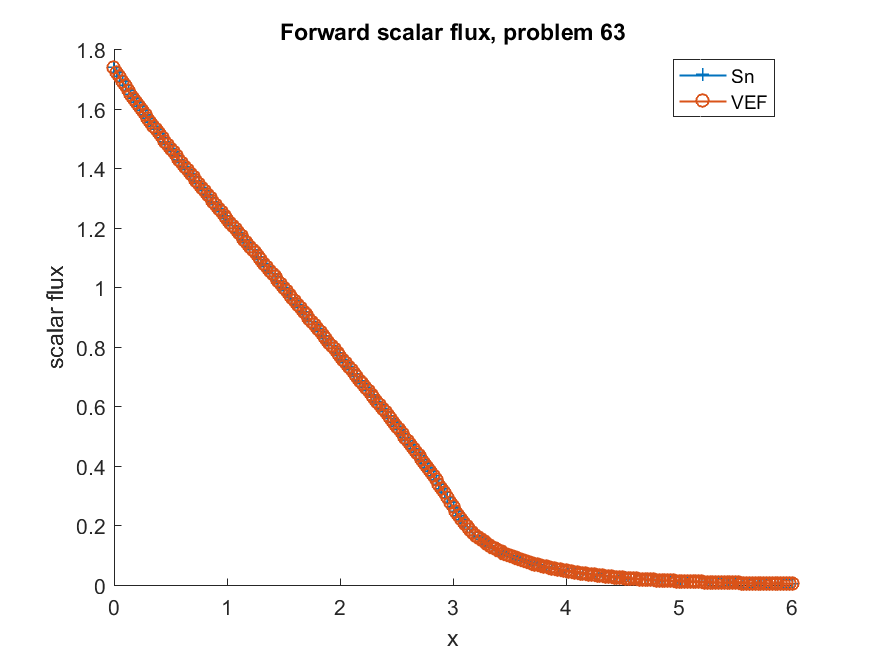
\includegraphics[width=.98\linewidth]{IanProposal/figures2/63phi.png}
  \caption{Forward flux}
  \label{fig:sfig1}
\end{subfigure}%
\begin{subfigure}{.5\textwidth}
  \centering
  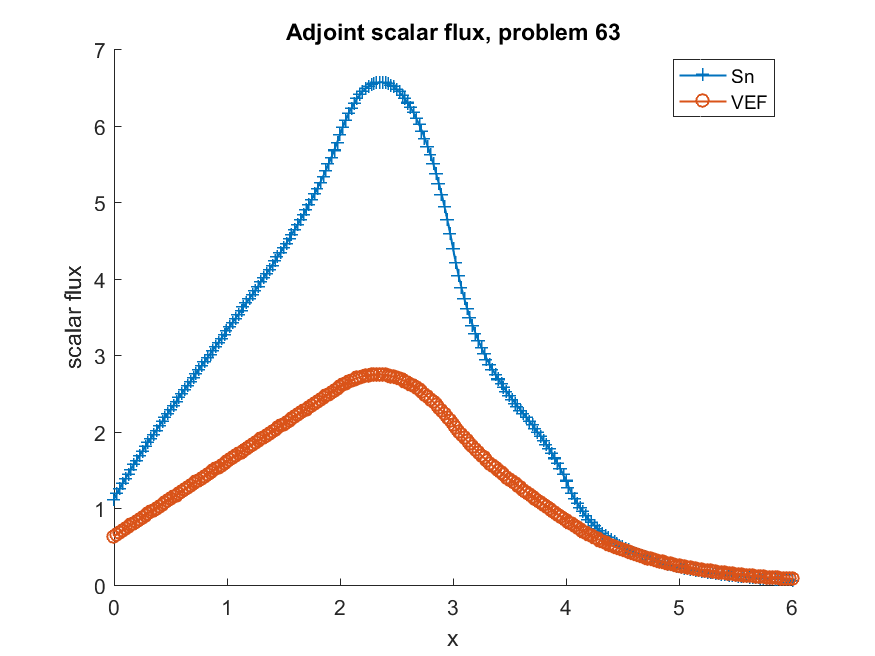
\includegraphics[width=.98\linewidth]{IanProposal/figures2/63phia.png}
  \caption{Response flux}
  \label{fig:sfig4}
\end{subfigure}%
\end{figure}


\begin{figure}[H]
\label{Case63Sens}
\centering
\begin{subfigure}{.5\textwidth}
  \centering
  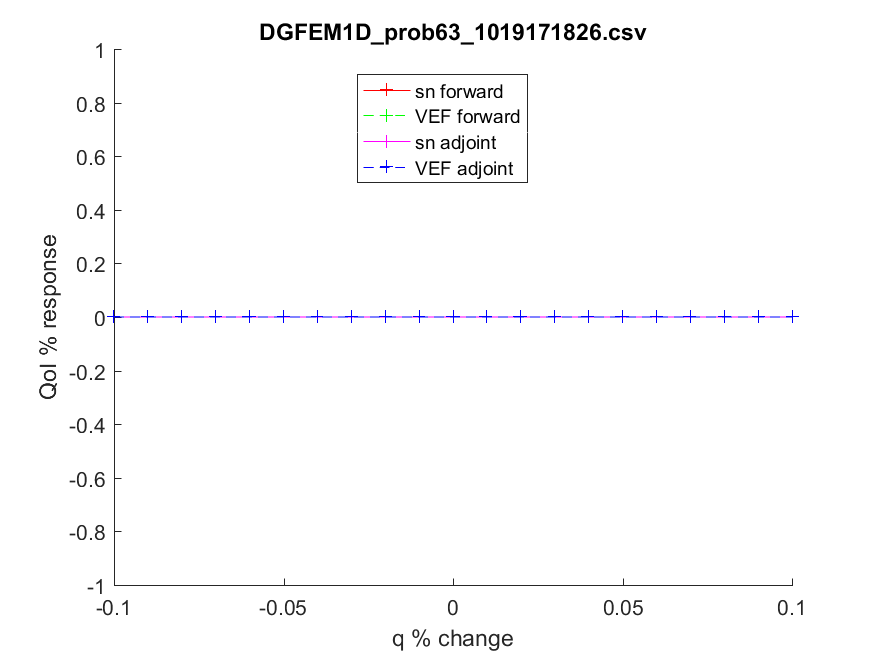
\includegraphics[width=.98\linewidth]{IanProposal/figures2/63qSens.png}
  \caption{Source sensitivity}
  \label{fig:sfig1}
\end{subfigure}%
\begin{subfigure}{.5\textwidth}
  \centering
  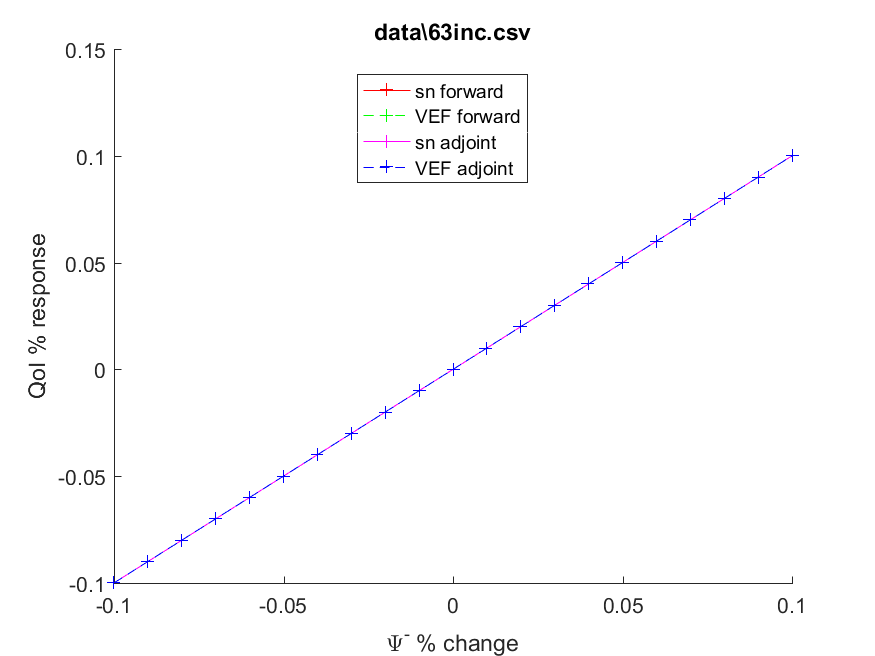
\includegraphics[width=.98\linewidth]{IanProposal/figures2/63incSens.png}
  \caption{Incident flux sensitivity}
  \label{fig:sfig4}
\end{subfigure}%
\\
\begin{subfigure}{.5\textwidth}
  \centering
  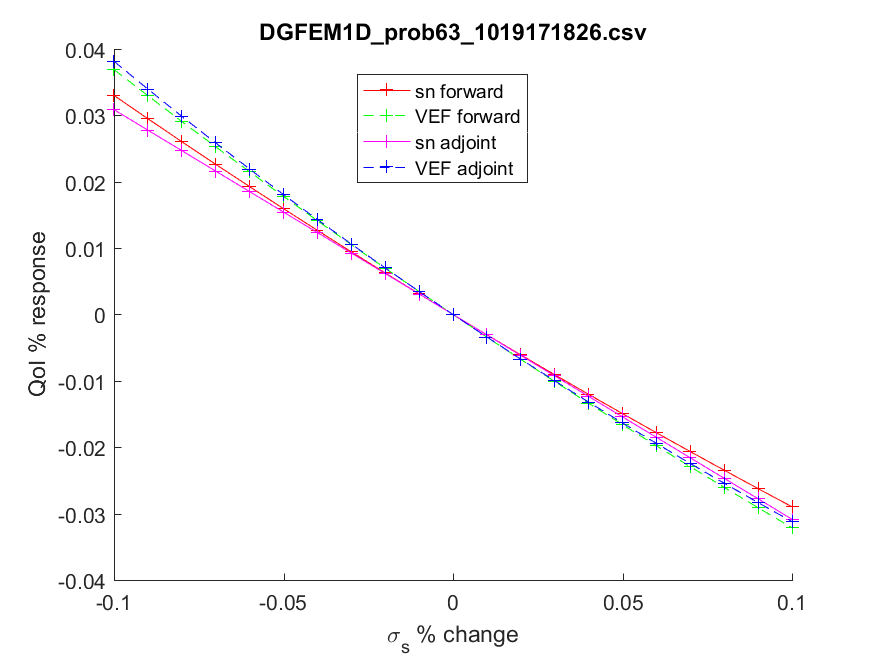
\includegraphics[width=.98\linewidth]{IanProposal/figures2/63sigsSens.png}
  \caption{Scattering cross-section sensitivity}
  \label{fig:sfig2}
\end{subfigure}%
\begin{subfigure}{.5\textwidth}
  \centering
  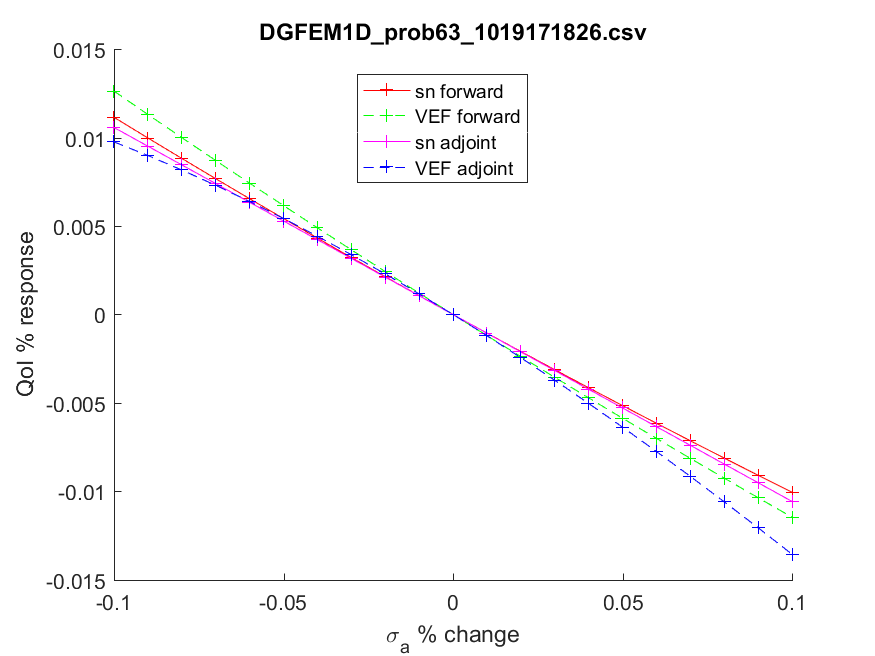
\includegraphics[width=.98\linewidth]{IanProposal/figures2/63sigaSens.png}
  \caption{Absorption cross-section sensitivity}
  \label{fig:sfig5}
\end{subfigure}%
\caption{}
\label{fig:fig}
\end{figure}
\newpage

%%%%%%%%%%%%%%%%%%%%%%%%%%%%%%%%%%%%%%%%%%%%%%%%%%%%%%
%%%%%%%%%%%%%%%%%%%%%%%%%%%%%%%%%%%%%%%%%%%%%%%%%%%%%%
%%%%%%%%%%%%%%%%%%%%%%%%%%%%%%%%%%%%%%%%%%%%%%%%%%%%%%
\subsection{64. Scat to abs}
\begin{verbatim}
case 64 %
        % number of elements per zone
        nel_zone = [ 10 10 10 10 10 10]*4;
        % width of each zone
        width_zone = [1 1 1 1 1 1];
        % sigt/sigs per zone
        sigt=[1 1 1 1 1 1];
        sigs=[1 1 1 0 0 0];
        % volumetric source value, per zone
        qvf=[0 0 0 0 0 0];
        % incoming flux values
        incf(1:sn) = 0;
        incf((sn/2)+1:sn) = 1;
        % volumetric response value, per zone
        qva=[0 1 1 0 0 0];
        % incoming adj flux values
        inca(1:sn) = 0;
        %Regions to be perturbed. Use value of 1 to specify
        dat.sigaPertRegion=[0 0 0 1 1 1];
        dat.sigsPertRegion=[1 1 1 0 0 0];
        dat.sourcePertRegion=[0 0 0 0 0 0];
        dat.incPertRegion(1:sn) = 1; 
        
-----BEGIN UNPERTURBED QOI DATA OUTPUT----- 
qoi using sn forward: 	 1.5282 
qoi using sn adjoint: 	 1.5282 
qoi using VEF forward: 	 1.52819 
qoi using VEF adjoint: 	 1.52819 
\end{verbatim}

\begin{figure}[H]
\label{Case64Flux}
\centering
\begin{subfigure}{.5\textwidth}
  \centering
  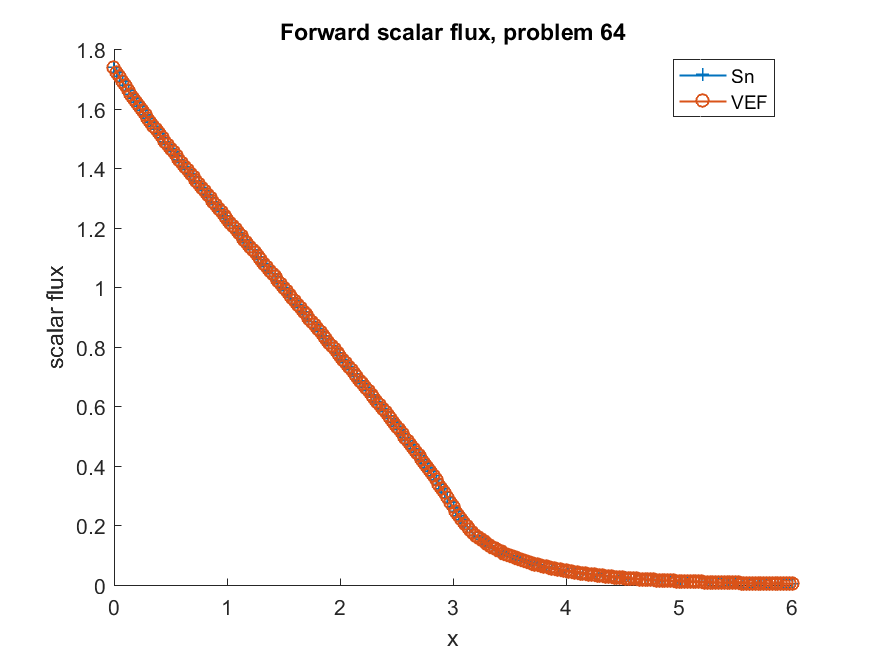
\includegraphics[width=.98\linewidth]{IanProposal/figures2/64phi.png}
  \caption{Forward flux}
  \label{fig:sfig1}
\end{subfigure}%
\begin{subfigure}{.5\textwidth}
  \centering
  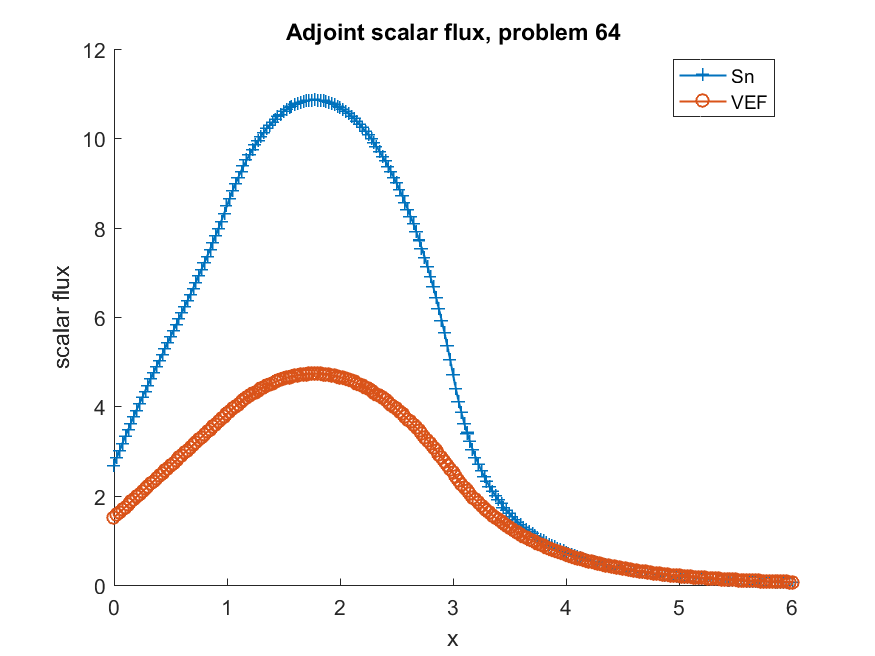
\includegraphics[width=.98\linewidth]{IanProposal/figures2/64phia.png}
  \caption{Response flux}
  \label{fig:sfig4}
\end{subfigure}%
\end{figure}


\begin{figure}[H]
\label{Case64Sens}
\centering
\begin{subfigure}{.5\textwidth}
  \centering
  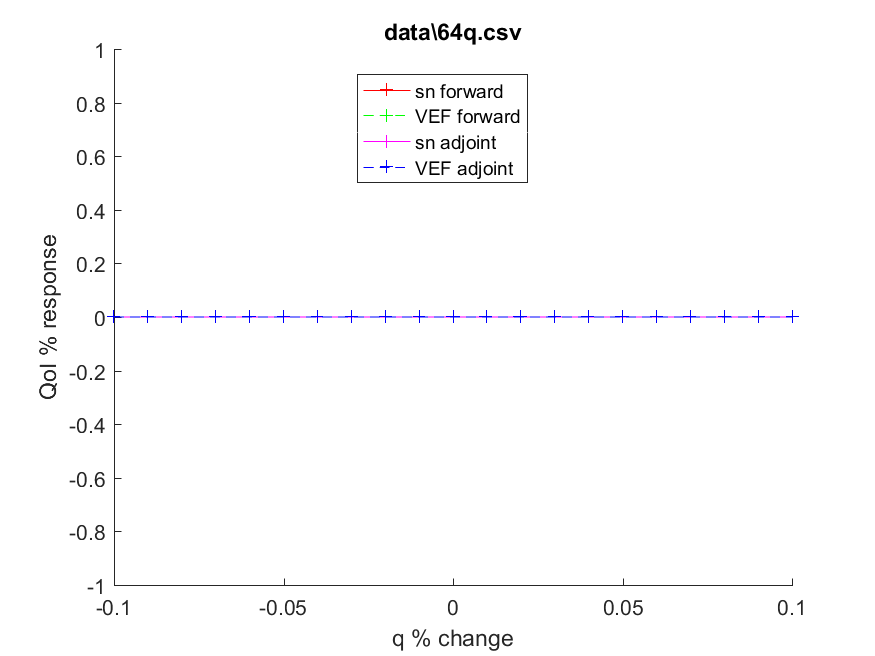
\includegraphics[width=.98\linewidth]{IanProposal/figures2/64qSens.png}
  \caption{Source sensitivity}
  \label{fig:sfig1}
\end{subfigure}%
\begin{subfigure}{.5\textwidth}
  \centering
  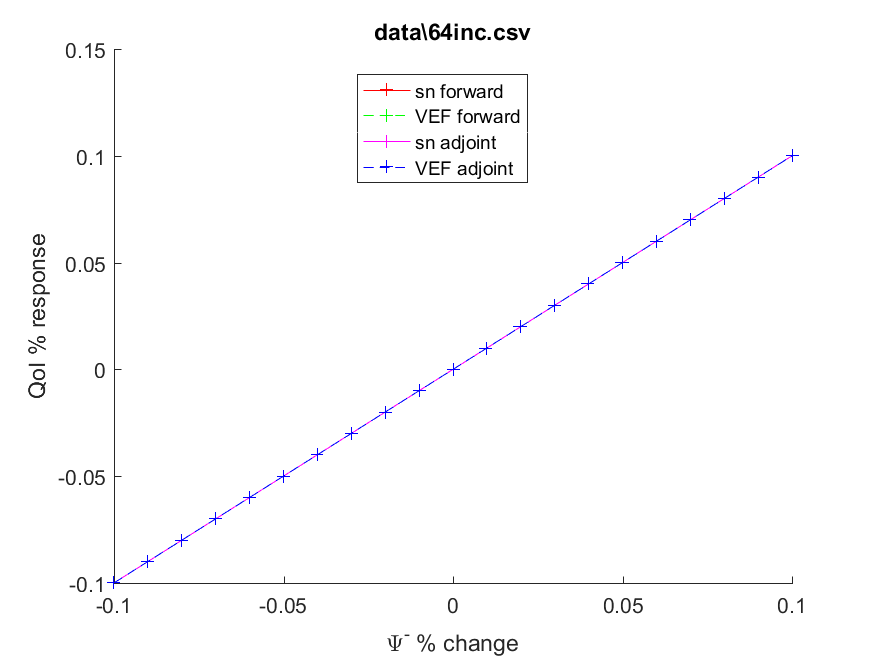
\includegraphics[width=.98\linewidth]{IanProposal/figures2/64incSens.png}
  \caption{Incident flux sensitivity}
  \label{fig:sfig4}
\end{subfigure}%
\\
\begin{subfigure}{.5\textwidth}
  \centering
  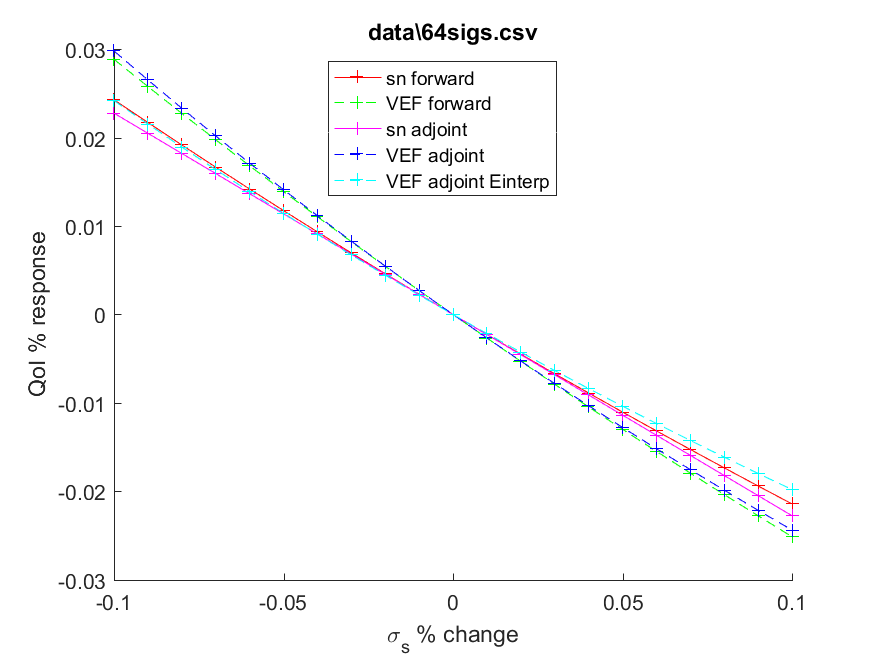
\includegraphics[width=.98\linewidth]{IanProposal/figures2/64sigsSens.png}
  \caption{Scattering cross-section sensitivity}
  \label{fig:sfig2}
\end{subfigure}%
\begin{subfigure}{.5\textwidth}
  \centering
  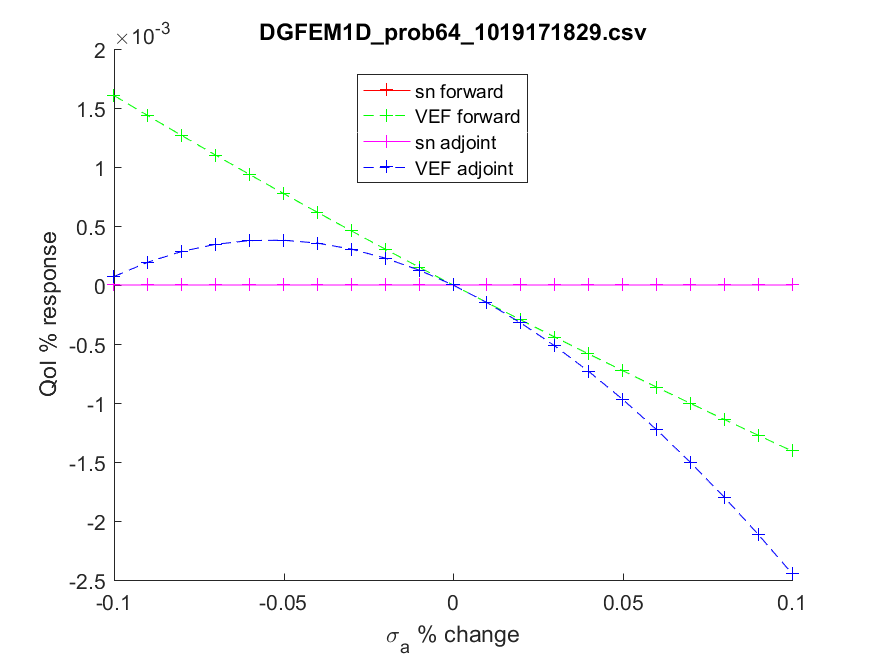
\includegraphics[width=.98\linewidth]{IanProposal/figures2/64sigaSens.png}
  \caption{Absorption cross-section sensitivity}
  \label{fig:sfig5}
\end{subfigure}%
\caption{}
\label{fig:fig}
\end{figure}
\newpage

%%%%%%%%%%%%%%%%%%%%%%%%%%%%%%%%%%%%%%%%%%%%%%%%%%%%%%
%%%%%%%%%%%%%%%%%%%%%%%%%%%%%%%%%%%%%%%%%%%%%%%%%%%%%%
%%%%%%%%%%%%%%%%%%%%%%%%%%%%%%%%%%%%%%%%%%%%%%%%%%%%%%
\subsection{65. Scat to abs}
\begin{verbatim}
case 65 %
        % number of elements per zone
        nel_zone = [ 10 10 10 10 10 10]*4;
        % width of each zone
        width_zone = [1 1 1 1 1 1];
        % sigt/sigs per zone
        sigt=[1 1 1 1 1 1];
        sigs=[1 1 1 0 0 0];
        % volumetric source value, per zone
        qvf=[0 0 0 0 0 0];
        % incoming flux values
        incf(1:sn) = 0;
        incf((sn/2)+1:sn) = 1;
        % volumetric response value, per zone
        qva=[0 0 0 1 1 0];
        % incoming adj flux values
        inca(1:sn) = 0;
        %Regions to be perturbed. Use value of 1 to specify
        dat.sigaPertRegion=[0 0 0 1 1 1];
        dat.sigsPertRegion=[1 1 1 0 0 0];
        dat.sourcePertRegion=[0 0 0 0 0 0];
        dat.incPertRegion(1:sn) = 1; 
        
-----BEGIN UNPERTURBED QOI DATA OUTPUT----- 
qoi using sn forward: 	 0.140839 
qoi using sn adjoint: 	 0.140839 
qoi using VEF forward: 	 0.140844 
qoi using VEF adjoint: 	 0.140844 
\end{verbatim}

\begin{figure}[H]
\label{Case65Flux}
\centering
\begin{subfigure}{.5\textwidth}
  \centering
  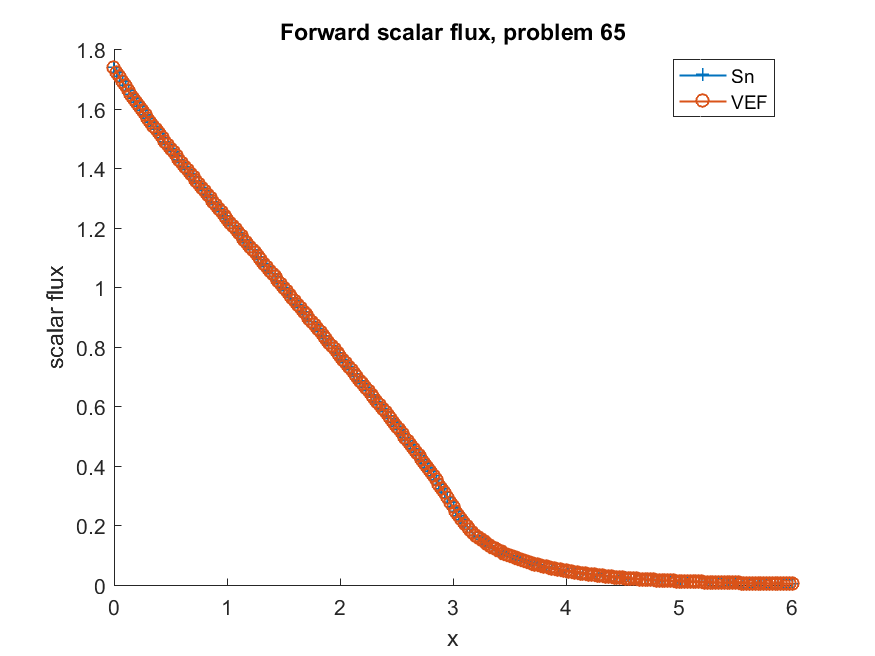
\includegraphics[width=.98\linewidth]{IanProposal/figures2/65phi.png}
  \caption{Forward flux}
  \label{fig:sfig1}
\end{subfigure}%
\begin{subfigure}{.5\textwidth}
  \centering
  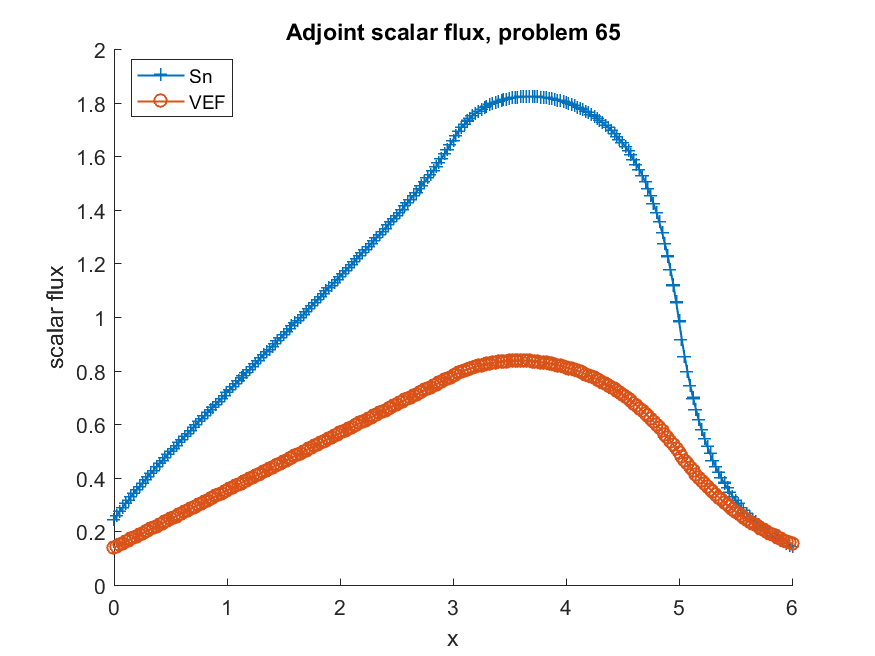
\includegraphics[width=.98\linewidth]{IanProposal/figures2/65phia.png}
  \caption{Response flux}
  \label{fig:sfig4}
\end{subfigure}%
\end{figure}


\begin{figure}[H]
\label{Case65Sens}
\centering
\begin{subfigure}{.5\textwidth}
  \centering
  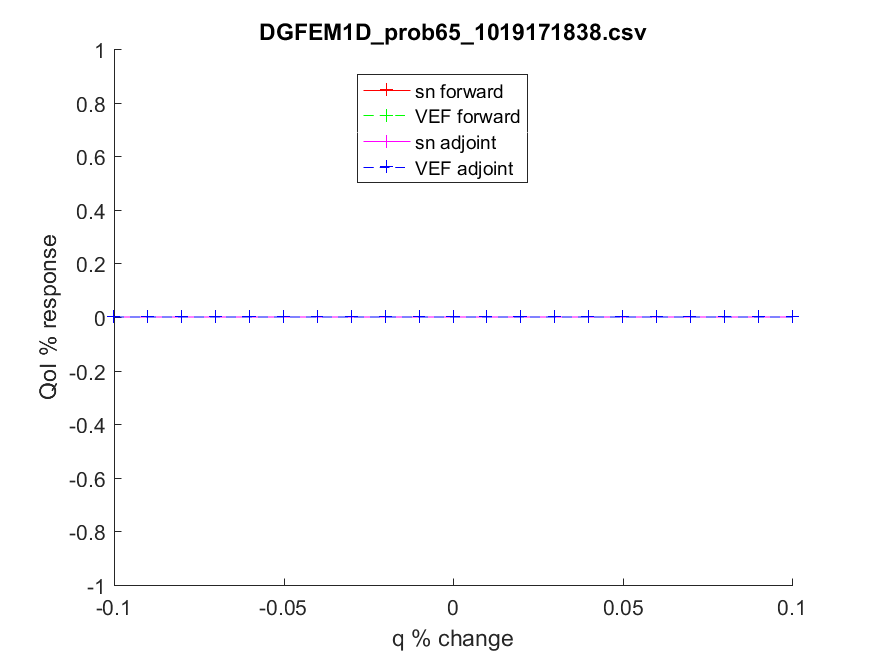
\includegraphics[width=.98\linewidth]{IanProposal/figures2/65qSens.png}
  \caption{Source sensitivity}
  \label{fig:sfig1}
\end{subfigure}%
\begin{subfigure}{.5\textwidth}
  \centering
  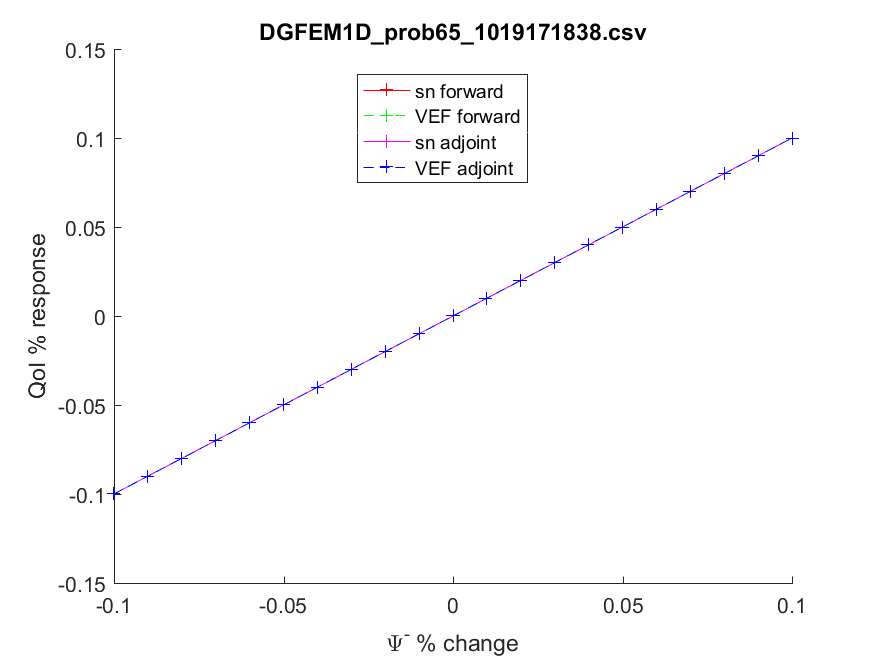
\includegraphics[width=.98\linewidth]{IanProposal/figures2/65incSens.png}
  \caption{Incident flux sensitivity}
  \label{fig:sfig4}
\end{subfigure}%
\\
\begin{subfigure}{.5\textwidth}
  \centering
  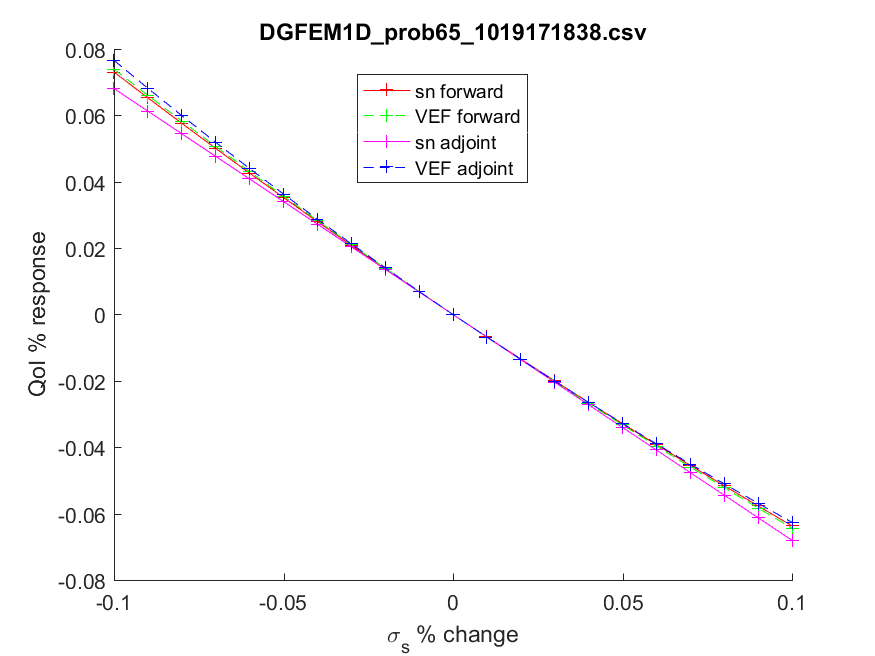
\includegraphics[width=.98\linewidth]{IanProposal/figures2/65sigsSens.png}
  \caption{Scattering cross-section sensitivity}
  \label{fig:sfig2}
\end{subfigure}%
\begin{subfigure}{.5\textwidth}
  \centering
  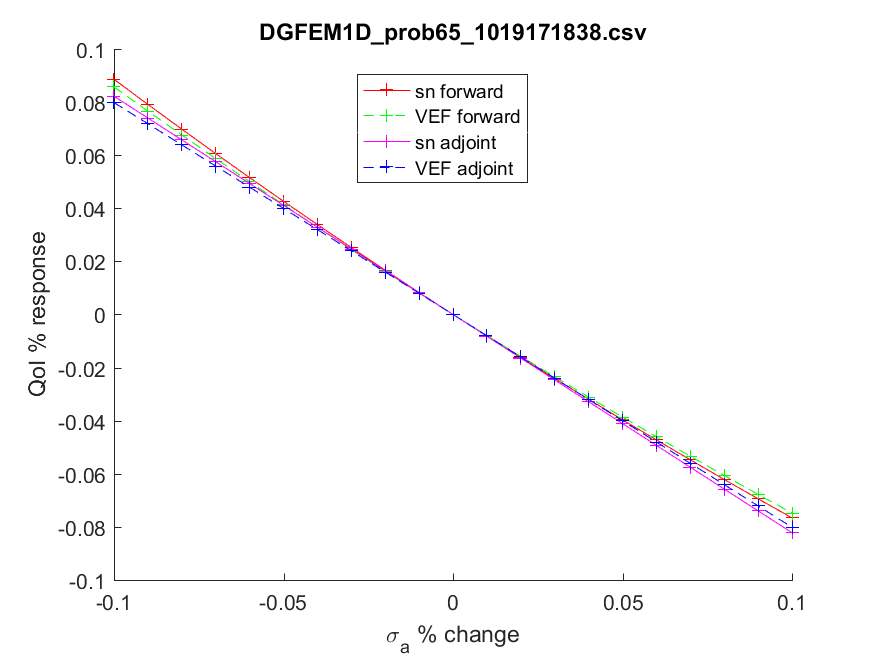
\includegraphics[width=.98\linewidth]{IanProposal/figures2/65sigaSens.png}
  \caption{Absorption cross-section sensitivity}
  \label{fig:sfig5}
\end{subfigure}%
\caption{}
\label{fig:fig}
\end{figure}
\newpage

%%%%%%%%%%%%%%%%%%%%%%%%%%%%%%%%%%%%%%%%%%%%%%%%%%%%%%
%%%%%%%%%%%%%%%%%%%%%%%%%%%%%%%%%%%%%%%%%%%%%%%%%%%%%%
%%%%%%%%%%%%%%%%%%%%%%%%%%%%%%%%%%%%%%%%%%%%%%%%%%%%%%
\subsection{66. Scat to scat}
\begin{verbatim}
case 66 %
        % number of elements per zone
        nel_zone = [ 10 10 10 10 10 10]*4;
        % width of each zone
        width_zone = [1 1 1 1 1 1];
        % sigt/sigs per zone
        sigt=[1 1 1 1 1 1];
        sigs=[1 1 1 1 1 1];
        % volumetric source value, per zone
        qvf=[0 0 0 0 0 0];
        % incoming flux values
        incf(1:sn) = 0;
        incf((sn/2)+1:sn) = 1;
        % volumetric response value, per zone
        qva=[0 0 1 1 0 0];
        % incoming adj flux values
        inca(1:sn) = 0;
        %Regions to be perturbed. Use value of 1 to specify
        dat.sigaPertRegion=[0 0 0 0 0 0];
        dat.sigsPertRegion=[1 1 1 0 0 0];
        dat.sourcePertRegion=[0 0 0 0 0 0];
        dat.incPertRegion(1:sn) = 1; 
        
-----BEGIN UNPERTURBED QOI DATA OUTPUT----- 
qoi using sn forward: 	 2 
qoi using sn adjoint: 	 2 
qoi using VEF forward: 	 2 
qoi using VEF adjoint: 	 2 
\end{verbatim}

\begin{figure}[H]
\label{Case66Flux}
\centering
\begin{subfigure}{.5\textwidth}
  \centering
  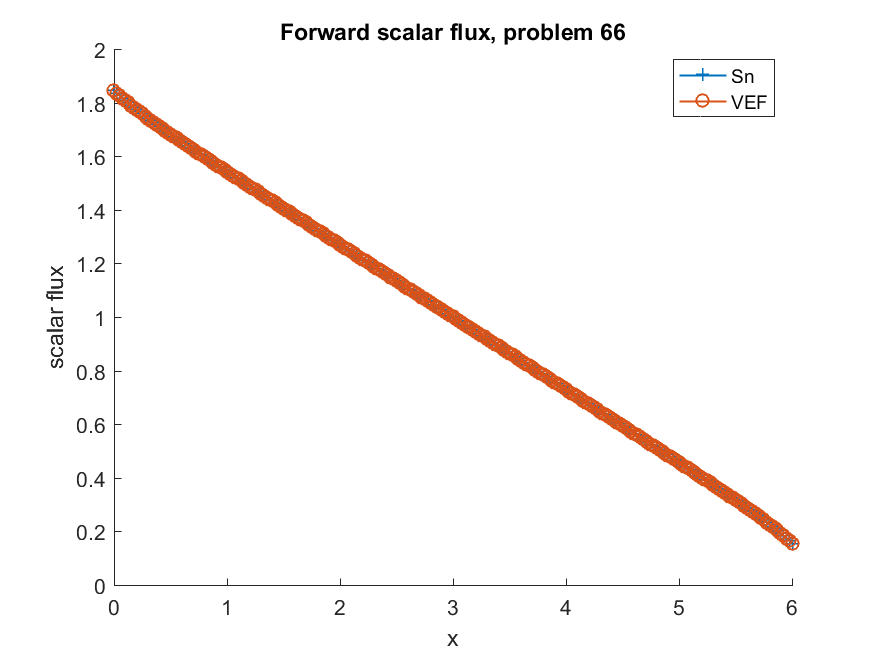
\includegraphics[width=.98\linewidth]{IanProposal/figures2/66phi.png}
  \caption{Forward flux}
  \label{fig:sfig1}
\end{subfigure}%
\begin{subfigure}{.5\textwidth}
  \centering
  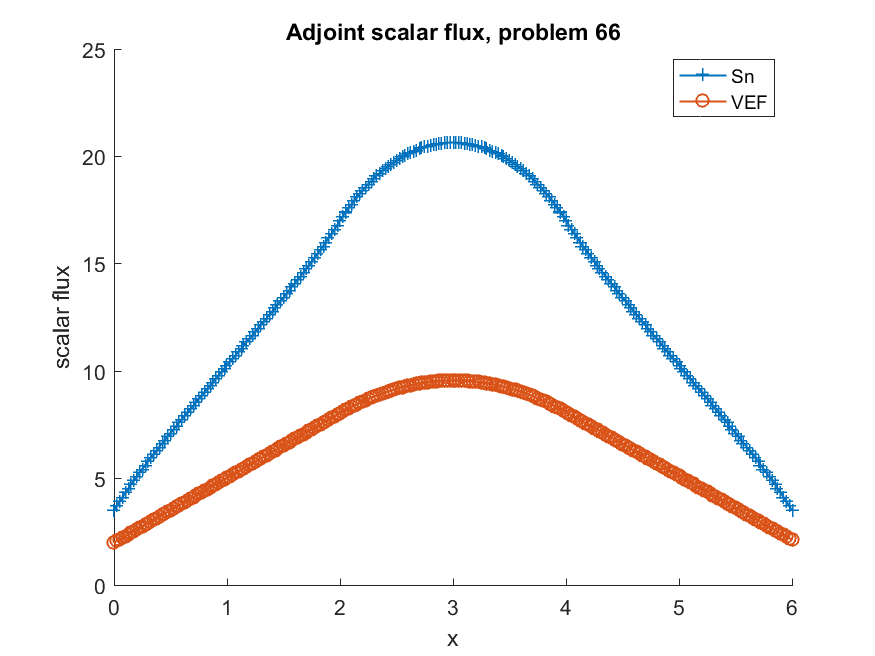
\includegraphics[width=.98\linewidth]{IanProposal/figures2/66phia.png}
  \caption{Response flux}
  \label{fig:sfig4}
\end{subfigure}%
\end{figure}


\begin{figure}[H]
\label{Case66Sens}
\centering
\begin{subfigure}{.5\textwidth}
  \centering
  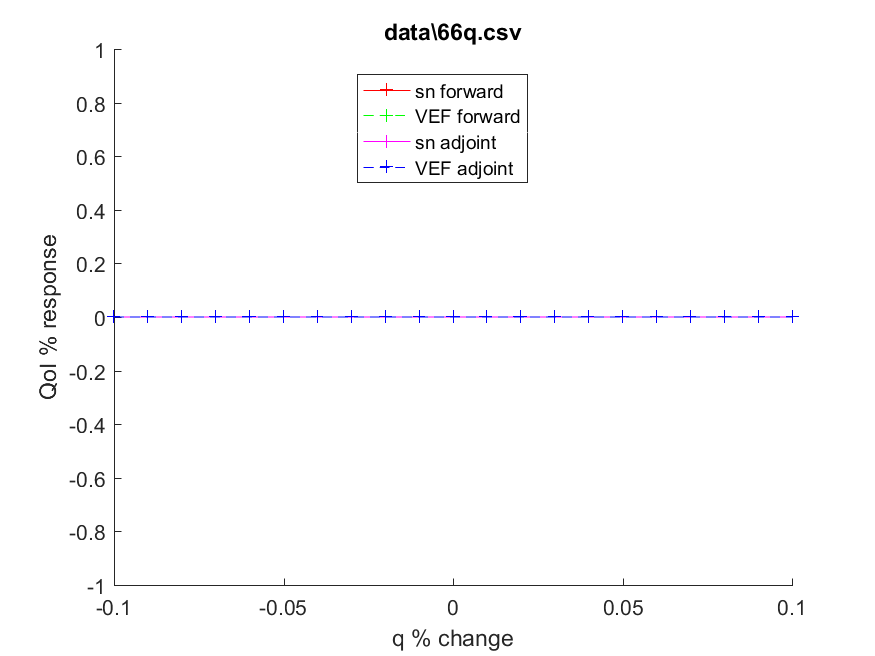
\includegraphics[width=.98\linewidth]{IanProposal/figures2/66qSens.png}
  \caption{Source sensitivity}
  \label{fig:sfig1}
\end{subfigure}%
\begin{subfigure}{.5\textwidth}
  \centering
  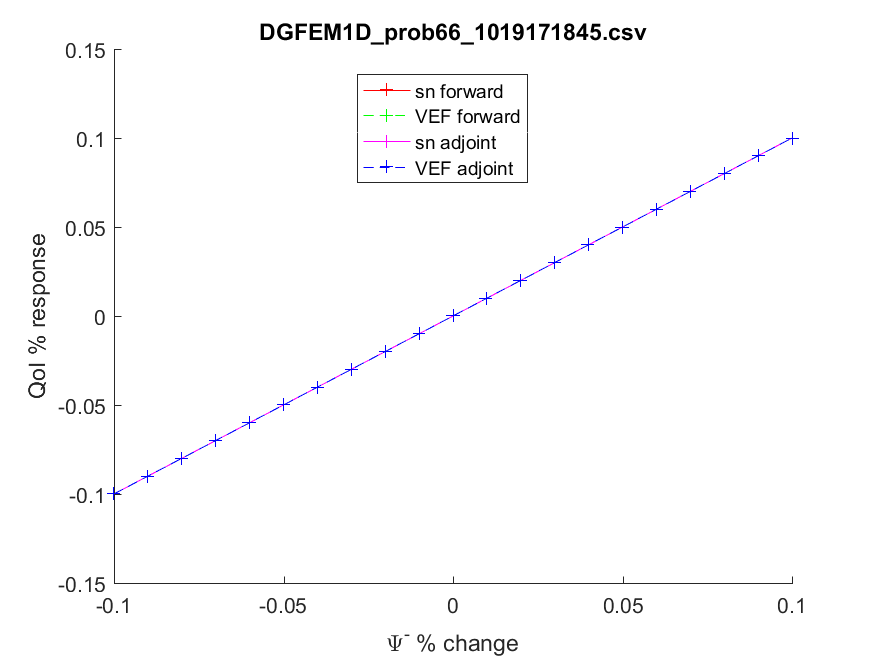
\includegraphics[width=.98\linewidth]{IanProposal/figures2/66incSens.png}
  \caption{Incident flux sensitivity}
  \label{fig:sfig4}
\end{subfigure}%
\\
\begin{subfigure}{.5\textwidth}
  \centering
  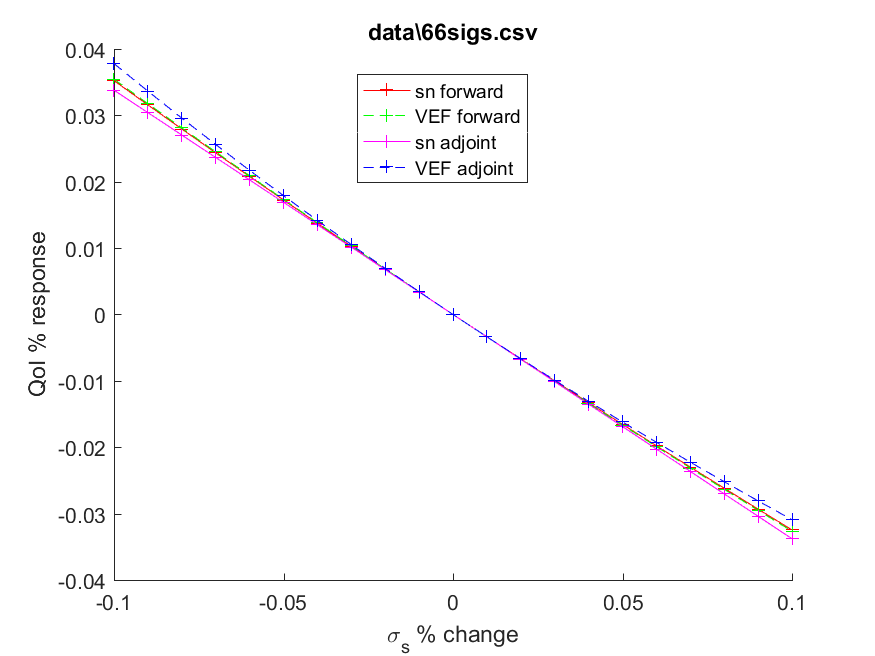
\includegraphics[width=.98\linewidth]{IanProposal/figures2/66sigsSens.png}
  \caption{Scattering cross-section sensitivity}
  \label{fig:sfig2}
\end{subfigure}%
\begin{subfigure}{.5\textwidth}
  \centering
  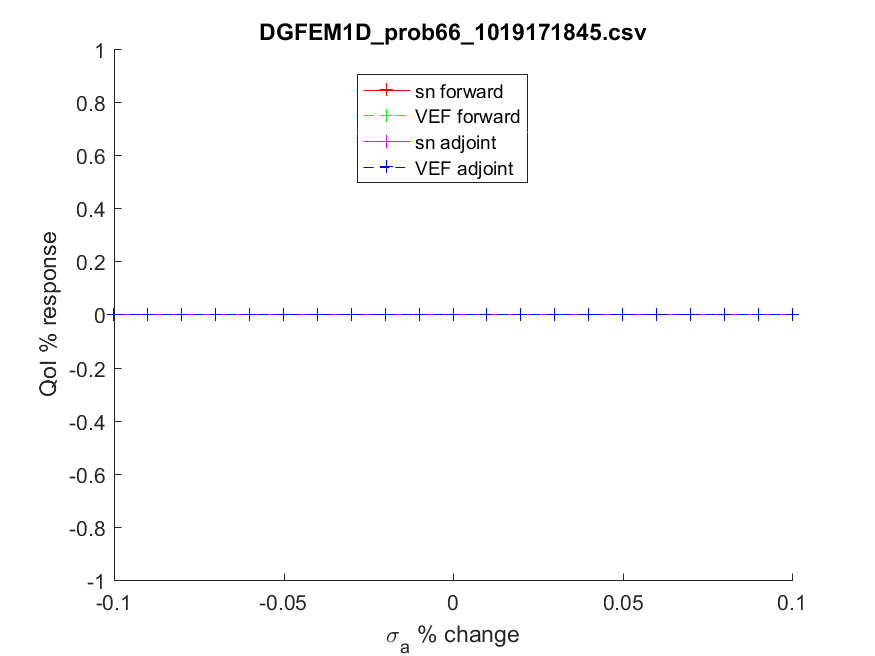
\includegraphics[width=.98\linewidth]{IanProposal/figures2/66sigaSens.png}
  \caption{Absorption cross-section sensitivity}
  \label{fig:sfig5}
\end{subfigure}%
\caption{}
\label{fig:fig}
\end{figure}
\newpage


%%%%%%%%%%%%%%%%%%%%%%%%%%%%%%%%%%%%%%%%%%%%%%%%%%%%%%
%%%%%%%%%%%%%%%%%%%%%%%%%%%%%%%%%%%%%%%%%%%%%%%%%%%%%%
%%%%%%%%%%%%%%%%%%%%%%%%%%%%%%%%%%%%%%%%%%%%%%%%%%%%%%
\subsection{67. Scat to scat}
\begin{verbatim}
case 67 %
        % number of elements per zone
        nel_zone = [ 10 10 10 10 10 10]*4;
        % width of each zone
        width_zone = [1 1 1 1 1 1];
        % sigt/sigs per zone
        sigt=[1 1 1 1 1 1];
        sigs=[1 1 1 1 1 1];
        % volumetric source value, per zone
        qvf=[0 0 0 0 0 0];
        % incoming flux values
        incf(1:sn) = 0;
        incf((sn/2)+1:sn) = 1;
        % volumetric response value, per zone
        qva=[0 1 1 0 0 0];
        % incoming adj flux values
        inca(1:sn) = 0;
        %Regions to be perturbed. Use value of 1 to specify
        dat.sigaPertRegion=[0 0 0 0 0 0];
        dat.sigsPertRegion=[1 1 1 0 0 0];
        dat.sourcePertRegion=[0 0 0 0 0 0];
        dat.incPertRegion(1:sn) = 1; 
        
-----BEGIN UNPERTURBED QOI DATA OUTPUT----- 
qoi using sn forward: 	 2.54135 
qoi using sn adjoint: 	 2.54135 
qoi using VEF forward: 	 2.54135 
qoi using VEF adjoint: 	 2.54135 
\end{verbatim}

\begin{figure}[H]
\label{Case67Flux}
\centering
\begin{subfigure}{.5\textwidth}
  \centering
  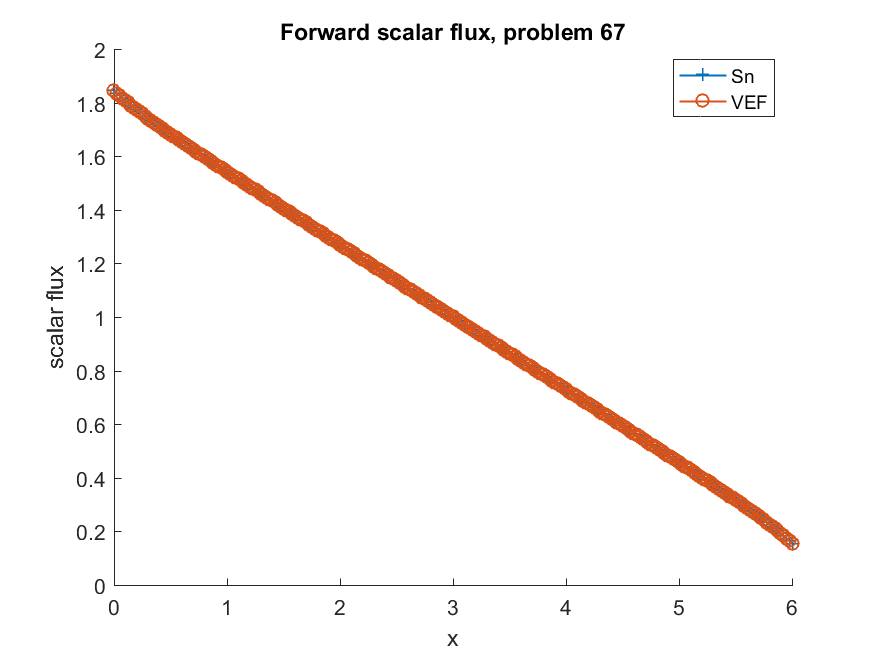
\includegraphics[width=.98\linewidth]{IanProposal/figures2/67phi.png}
  \caption{Forward flux}
  \label{fig:sfig1}
\end{subfigure}%
\begin{subfigure}{.5\textwidth}
  \centering
  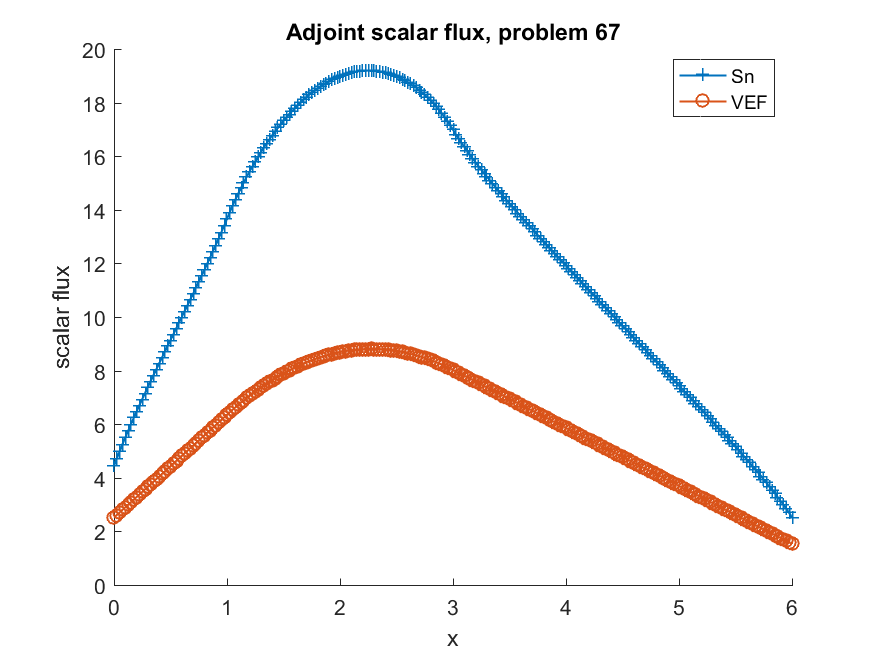
\includegraphics[width=.98\linewidth]{IanProposal/figures2/67phia.png}
  \caption{Response flux}
  \label{fig:sfig4}
\end{subfigure}%
\end{figure}


\begin{figure}[H]
\label{Case67Sens}
\centering
\begin{subfigure}{.5\textwidth}
  \centering
  \includegraphics[width=.98\linewidth]{IanProposal/figures2/67qSens.png}
  \caption{Source sensitivity}
  \label{fig:sfig1}
\end{subfigure}%
\begin{subfigure}{.5\textwidth}
  \centering
  \includegraphics[width=.98\linewidth]{IanProposal/figures2/67incSens.png}
  \caption{Incident flux sensitivity}
  \label{fig:sfig4}
\end{subfigure}%
\\
\begin{subfigure}{.5\textwidth}
  \centering
  \includegraphics[width=.98\linewidth]{IanProposal/figures2/67sigsSens.png}
  \caption{Scattering cross-section sensitivity}
  \label{fig:sfig2}
\end{subfigure}%
\begin{subfigure}{.5\textwidth}
  \centering
  \includegraphics[width=.98\linewidth]{IanProposal/figures2/67sigaSens.png}
  \caption{Absorption cross-section sensitivity}
  \label{fig:sfig5}
\end{subfigure}%
\caption{}
\label{fig:fig}
\end{figure}
\newpage

%%%%%%%%%%%%%%%%%%%%%%%%%%%%%%%%%%%%%%%%%%%%%%%%%%%%%%
%%%%%%%%%%%%%%%%%%%%%%%%%%%%%%%%%%%%%%%%%%%%%%%%%%%%%%
%%%%%%%%%%%%%%%%%%%%%%%%%%%%%%%%%%%%%%%%%%%%%%%%%%%%%%
\subsection{68. Scat to scat}
\begin{verbatim}
case 68 %
        % number of elements per zone
        nel_zone = [ 10 10 10 10 10 10]*4;
        % width of each zone
        width_zone = [1 1 1 1 1 1];
        % sigt/sigs per zone
        sigt=[1 1 1 1 1 1];
        sigs=[1 1 1 1 1 1];
        % volumetric source value, per zone
        qvf=[0 0 0 0 0 0];
        % incoming flux values
        incf(1:sn) = 0;
        incf((sn/2)+1:sn) = 1;
        % volumetric response value, per zone
        qva=[0 0 0 1 1 0];
        % incoming adj flux values
        inca(1:sn) = 0;
        %Regions to be perturbed. Use value of 1 to specify
        dat.sigaPertRegion=[0 0 0 0 0 0];
        dat.sigsPertRegion=[1 1 1 0 0 0];
        dat.sourcePertRegion=[0 0 0 0 0 0];
        dat.incPertRegion(1:sn) = 1; 
        
-----BEGIN UNPERTURBED QOI DATA OUTPUT----- 
qoi using sn forward: 	 1.45865 
qoi using sn adjoint: 	 1.45865 
qoi using VEF forward: 	 1.45865 
qoi using VEF adjoint: 	 1.45865 
\end{verbatim}

\begin{figure}[H]
\label{Case68Flux}
\centering
\begin{subfigure}{.5\textwidth}
  \centering
  \includegraphics[width=.98\linewidth]{IanProposal/figures2/68phi.png}
  \caption{Forward flux}
  \label{fig:sfig1}
\end{subfigure}%
\begin{subfigure}{.5\textwidth}
  \centering
  \includegraphics[width=.98\linewidth]{IanProposal/figures2/68phia.png}
  \caption{Response flux}
  \label{fig:sfig4}
\end{subfigure}%
\end{figure}


\begin{figure}[H]
\label{Case68Sens}
\centering
\begin{subfigure}{.5\textwidth}
  \centering
  \includegraphics[width=.98\linewidth]{IanProposal/figures2/68qSens.png}
  \caption{Source sensitivity}
  \label{fig:sfig1}
\end{subfigure}%
\begin{subfigure}{.5\textwidth}
  \centering
  \includegraphics[width=.98\linewidth]{IanProposal/figures2/68incSens.png}
  \caption{Incident flux sensitivity}
  \label{fig:sfig4}
\end{subfigure}%
\\
\begin{subfigure}{.5\textwidth}
  \centering
  \includegraphics[width=.98\linewidth]{IanProposal/figures2/68sigsSens.png}
  \caption{Scattering cross-section sensitivity}
  \label{fig:sfig2}
\end{subfigure}%
\begin{subfigure}{.5\textwidth}
  \centering
  \includegraphics[width=.98\linewidth]{IanProposal/figures2/68sigaSens.png}
  \caption{Absorption cross-section sensitivity}
  \label{fig:sfig5}
\end{subfigure}%
\caption{}
\label{fig:fig}
\end{figure}
\newpage

\end{document}